\documentclass[]{article}
\usepackage{lmodern}
\usepackage{amssymb,amsmath}
\usepackage{ifxetex,ifluatex}
\usepackage{fixltx2e} % provides \textsubscript
\ifnum 0\ifxetex 1\fi\ifluatex 1\fi=0 % if pdftex
  \usepackage[T1]{fontenc}
  \usepackage[utf8]{inputenc}
\else % if luatex or xelatex
  \ifxetex
    \usepackage{mathspec}
  \else
    \usepackage{fontspec}
  \fi
  \defaultfontfeatures{Ligatures=TeX,Scale=MatchLowercase}
\fi
% use upquote if available, for straight quotes in verbatim environments
\IfFileExists{upquote.sty}{\usepackage{upquote}}{}
% use microtype if available
\IfFileExists{microtype.sty}{%
\usepackage{microtype}
\UseMicrotypeSet[protrusion]{basicmath} % disable protrusion for tt fonts
}{}
\usepackage[margin=1in]{geometry}
\usepackage{hyperref}
\hypersetup{unicode=true,
            pdftitle={Data Cleaning and Preliminary Analysis},
            pdfauthor={Dionna Attinson},
            pdfborder={0 0 0},
            breaklinks=true}
\urlstyle{same}  % don't use monospace font for urls
\usepackage{color}
\usepackage{fancyvrb}
\newcommand{\VerbBar}{|}
\newcommand{\VERB}{\Verb[commandchars=\\\{\}]}
\DefineVerbatimEnvironment{Highlighting}{Verbatim}{commandchars=\\\{\}}
% Add ',fontsize=\small' for more characters per line
\usepackage{framed}
\definecolor{shadecolor}{RGB}{248,248,248}
\newenvironment{Shaded}{\begin{snugshade}}{\end{snugshade}}
\newcommand{\AlertTok}[1]{\textcolor[rgb]{0.94,0.16,0.16}{#1}}
\newcommand{\AnnotationTok}[1]{\textcolor[rgb]{0.56,0.35,0.01}{\textbf{\textit{#1}}}}
\newcommand{\AttributeTok}[1]{\textcolor[rgb]{0.77,0.63,0.00}{#1}}
\newcommand{\BaseNTok}[1]{\textcolor[rgb]{0.00,0.00,0.81}{#1}}
\newcommand{\BuiltInTok}[1]{#1}
\newcommand{\CharTok}[1]{\textcolor[rgb]{0.31,0.60,0.02}{#1}}
\newcommand{\CommentTok}[1]{\textcolor[rgb]{0.56,0.35,0.01}{\textit{#1}}}
\newcommand{\CommentVarTok}[1]{\textcolor[rgb]{0.56,0.35,0.01}{\textbf{\textit{#1}}}}
\newcommand{\ConstantTok}[1]{\textcolor[rgb]{0.00,0.00,0.00}{#1}}
\newcommand{\ControlFlowTok}[1]{\textcolor[rgb]{0.13,0.29,0.53}{\textbf{#1}}}
\newcommand{\DataTypeTok}[1]{\textcolor[rgb]{0.13,0.29,0.53}{#1}}
\newcommand{\DecValTok}[1]{\textcolor[rgb]{0.00,0.00,0.81}{#1}}
\newcommand{\DocumentationTok}[1]{\textcolor[rgb]{0.56,0.35,0.01}{\textbf{\textit{#1}}}}
\newcommand{\ErrorTok}[1]{\textcolor[rgb]{0.64,0.00,0.00}{\textbf{#1}}}
\newcommand{\ExtensionTok}[1]{#1}
\newcommand{\FloatTok}[1]{\textcolor[rgb]{0.00,0.00,0.81}{#1}}
\newcommand{\FunctionTok}[1]{\textcolor[rgb]{0.00,0.00,0.00}{#1}}
\newcommand{\ImportTok}[1]{#1}
\newcommand{\InformationTok}[1]{\textcolor[rgb]{0.56,0.35,0.01}{\textbf{\textit{#1}}}}
\newcommand{\KeywordTok}[1]{\textcolor[rgb]{0.13,0.29,0.53}{\textbf{#1}}}
\newcommand{\NormalTok}[1]{#1}
\newcommand{\OperatorTok}[1]{\textcolor[rgb]{0.81,0.36,0.00}{\textbf{#1}}}
\newcommand{\OtherTok}[1]{\textcolor[rgb]{0.56,0.35,0.01}{#1}}
\newcommand{\PreprocessorTok}[1]{\textcolor[rgb]{0.56,0.35,0.01}{\textit{#1}}}
\newcommand{\RegionMarkerTok}[1]{#1}
\newcommand{\SpecialCharTok}[1]{\textcolor[rgb]{0.00,0.00,0.00}{#1}}
\newcommand{\SpecialStringTok}[1]{\textcolor[rgb]{0.31,0.60,0.02}{#1}}
\newcommand{\StringTok}[1]{\textcolor[rgb]{0.31,0.60,0.02}{#1}}
\newcommand{\VariableTok}[1]{\textcolor[rgb]{0.00,0.00,0.00}{#1}}
\newcommand{\VerbatimStringTok}[1]{\textcolor[rgb]{0.31,0.60,0.02}{#1}}
\newcommand{\WarningTok}[1]{\textcolor[rgb]{0.56,0.35,0.01}{\textbf{\textit{#1}}}}
\usepackage{longtable,booktabs}
\usepackage{graphicx,grffile}
\makeatletter
\def\maxwidth{\ifdim\Gin@nat@width>\linewidth\linewidth\else\Gin@nat@width\fi}
\def\maxheight{\ifdim\Gin@nat@height>\textheight\textheight\else\Gin@nat@height\fi}
\makeatother
% Scale images if necessary, so that they will not overflow the page
% margins by default, and it is still possible to overwrite the defaults
% using explicit options in \includegraphics[width, height, ...]{}
\setkeys{Gin}{width=\maxwidth,height=\maxheight,keepaspectratio}
\IfFileExists{parskip.sty}{%
\usepackage{parskip}
}{% else
\setlength{\parindent}{0pt}
\setlength{\parskip}{6pt plus 2pt minus 1pt}
}
\setlength{\emergencystretch}{3em}  % prevent overfull lines
\providecommand{\tightlist}{%
  \setlength{\itemsep}{0pt}\setlength{\parskip}{0pt}}
\setcounter{secnumdepth}{0}
% Redefines (sub)paragraphs to behave more like sections
\ifx\paragraph\undefined\else
\let\oldparagraph\paragraph
\renewcommand{\paragraph}[1]{\oldparagraph{#1}\mbox{}}
\fi
\ifx\subparagraph\undefined\else
\let\oldsubparagraph\subparagraph
\renewcommand{\subparagraph}[1]{\oldsubparagraph{#1}\mbox{}}
\fi

%%% Use protect on footnotes to avoid problems with footnotes in titles
\let\rmarkdownfootnote\footnote%
\def\footnote{\protect\rmarkdownfootnote}

%%% Change title format to be more compact
\usepackage{titling}

% Create subtitle command for use in maketitle
\providecommand{\subtitle}[1]{
  \posttitle{
    \begin{center}\large#1\end{center}
    }
}

\setlength{\droptitle}{-2em}

  \title{Data Cleaning and Preliminary Analysis}
    \pretitle{\vspace{\droptitle}\centering\huge}
  \posttitle{\par}
    \author{Dionna Attinson}
    \preauthor{\centering\large\emph}
  \postauthor{\par}
      \predate{\centering\large\emph}
  \postdate{\par}
    \date{2/7/2020}


\begin{document}
\maketitle

\begin{Shaded}
\begin{Highlighting}[]
\NormalTok{SurveyData =}\StringTok{ }
\StringTok{  }\NormalTok{readxl}\OperatorTok{::}\KeywordTok{read_xls}\NormalTok{(}\StringTok{'./SFH_Survey_CODED_CLEANED.xls'}\NormalTok{) }\OperatorTok\StringTok{ }
\StringTok{  }\NormalTok{janitor}\OperatorTok{::}\KeywordTok{clean_names}\NormalTok{()}
\end{Highlighting}
\end{Shaded}

\begin{verbatim}
## New names:
## * PSS_8 -> PSS_8...108
## * PSS_8 -> PSS_8...109
\end{verbatim}

\hypertarget{data-cleaning-and-recoding}{%
\subsubsection{Data Cleaning and
Recoding}\label{data-cleaning-and-recoding}}

\begin{Shaded}
\begin{Highlighting}[]
\NormalTok{SurveyData =}
\StringTok{ }\NormalTok{SurveyData }\OperatorTok\StringTok{ }
\StringTok{ }\KeywordTok{rename}\NormalTok{(}\DataTypeTok{Gender =}\NormalTok{ x1_to_which_gender_identity_do_you_most_identify_selected_choice,}
        \DataTypeTok{Education =}\NormalTok{ x3_what_is_the_highest_level_of_education_you_have_completed_selected_choice,}
        \DataTypeTok{Race =}\NormalTok{ x4_which_best_describes_your_race_ethnicity_check_all_that_apply_selected_choice,}
        \DataTypeTok{Income =}\NormalTok{ x7_hand_participant_income_card_which_of_these_groups_on_this_card_is_closest_to_your_total_personal_income_before_taxes_during_the_last_year_please_include_income_from_all_sources_your_salaries_wages_and_any_benefits_including_social_security_welfare_gifts_or_any_other_income_please_do_not_include_food_stamps_or_rental_subsidies_tell_me_the_code_for_the_amount_you_got_last_year_or_the_code_for_the_amount_you_usually_get_per_month_if_necessary_work_with_resident_to_construct_a_monthly_personal_and_household_income)}
\end{Highlighting}
\end{Shaded}

\hypertarget{in-the-code-chunk-below-a-number-of-variables-were-recoded-as-binary.}{%
\subparagraph{In the code chunk below, a number of variables were
recoded as
binary.}\label{in-the-code-chunk-below-a-number-of-variables-were-recoded-as-binary.}}

\begin{itemize}
\tightlist
\item
  \texttt{Smoke} was the variable that identified the smoking status of
  an individual. Those who responded that they smoke ANY products
  including marijuana, THC, hash, hookah, E-cigarettes, Cigarettes or
  Cigarillos were coded as \texttt{1} = Smoker. Those who responded that
  they did not smoke any products were coded as \texttt{0}, Non-smoker.
\item
  Evidence of mice/rats, cockroaches, and having a mildew odor present
  in the home were all coded as \texttt{1} = Yes, \texttt{0} = No.
\end{itemize}

\begin{Shaded}
\begin{Highlighting}[]
\NormalTok{VariablesofInterest =}\StringTok{ }
\StringTok{  }\NormalTok{SurveyData }\OperatorTok\StringTok{ }
\StringTok{  }\KeywordTok{select}\NormalTok{(age, Gender, Race, pss_}\DecValTok{5}\NormalTok{, pss_}\DecValTok{6}\NormalTok{, pss_}\DecValTok{8}\NormalTok{_}\DecValTok{108}\NormalTok{, pss_}\DecValTok{8}\NormalTok{_}\DecValTok{109}\NormalTok{, pss_}\DecValTok{10}\NormalTok{, sf36_}\DecValTok{1}\NormalTok{, sf36_}\DecValTok{4}\NormalTok{, }
\NormalTok{        sf36_}\DecValTok{6}\NormalTok{, sf36_}\DecValTok{14}\NormalTok{, sf36_}\DecValTok{15}\NormalTok{, sf36_}\DecValTok{18}\NormalTok{, sf36_}\DecValTok{19}\NormalTok{, sf36_}\DecValTok{22}\NormalTok{, sf36_}\DecValTok{26}\NormalTok{, sf36_}\DecValTok{27}\NormalTok{, sf36_}\DecValTok{28}\NormalTok{,}
\NormalTok{        sf36_}\DecValTok{32}\NormalTok{, Education, Income, repairs_needed, asthma, anxiety, lungd, depression,}
\NormalTok{        heartdisease, cancer, diabetes,hypertension, products_used, neg_health_building, }
\NormalTok{        micerats, cockroaches, mildew, homesat,buildsat, neighborhoodsat, propmansat) }\OperatorTok\StringTok{ }
\StringTok{  }
\StringTok{  }\KeywordTok{rename}\NormalTok{(}\DataTypeTok{Smoke =}\NormalTok{ products_used) }\OperatorTok\StringTok{ }
\StringTok{  }\KeywordTok{rename}\NormalTok{(}\DataTypeTok{Age =}\NormalTok{ age) }\OperatorTok\StringTok{ }
\StringTok{  }\KeywordTok{mutate}\NormalTok{(}\DataTypeTok{Smoke =} \KeywordTok{recode}\NormalTok{(Smoke, }
                    \StringTok{"Dont smoke"}\NormalTok{ =}\StringTok{ "0"}\NormalTok{,}
                    \StringTok{"Cigarettes and/or Cigarillos (common brands are Marlboro, Black & Mild)"}\NormalTok{ =}\StringTok{ "1"}\NormalTok{,}
                    \StringTok{"Hookah"}\NormalTok{ =}\StringTok{ "1"}\NormalTok{,}
                    \StringTok{"Cigarettes and/or Cigarillos (common brands are Marlboro, Black & Mild) ,Marijuana, hash, THC, grass, pot, or weed"}\NormalTok{ =}\StringTok{ "1"}\NormalTok{,}
                    \StringTok{"Cigarettes and/or Cigarillos (common brands are Marlboro, Black & Mild) ,E-cigarettes (look like regular cigarettes, but are battery-powered),Marijuana, hash, THC, grass, pot, or weed,Hookah"}\NormalTok{ =}\StringTok{ "1"}\NormalTok{,}
                    \StringTok{"E-cigarettes (look like regular cigarettes, but are battery-powered)"}\NormalTok{ =}\StringTok{ "1"}\NormalTok{,}
                   \StringTok{"Marijuana, hash, THC, grass, pot, or weed"}\NormalTok{ =}\StringTok{ "1"}\NormalTok{),}
        \DataTypeTok{micerats =} \KeywordTok{recode}\NormalTok{(micerats, }
                          \StringTok{"Yes"}\NormalTok{ =}\StringTok{ "1"}\NormalTok{, }
                          \StringTok{"No"}\NormalTok{ =}\StringTok{ "0"}\NormalTok{),}
        \DataTypeTok{cockroaches =} \KeywordTok{recode}\NormalTok{(cockroaches, }
                             \StringTok{"Yes"}\NormalTok{ =}\StringTok{ "1"}\NormalTok{, }
                             \StringTok{"No"}\NormalTok{ =}\StringTok{ "0"}\NormalTok{),}
        \DataTypeTok{mildew =} \KeywordTok{recode}\NormalTok{(mildew, }
                            \StringTok{"Yes"}\NormalTok{ =}\StringTok{ "1"}\NormalTok{,}
                            \StringTok{"No"}\NormalTok{ =}\StringTok{ "0"}\NormalTok{),}
        \DataTypeTok{neg_health_building =} \KeywordTok{recode}\NormalTok{(neg_health_building, }
                                      \StringTok{"Yes"}\NormalTok{ =}\StringTok{ "1"}\NormalTok{,}
                                      \StringTok{"No"}\NormalTok{ =}\StringTok{ "0"}\NormalTok{),}
        \DataTypeTok{Race =} \KeywordTok{recode}\NormalTok{(Race,}
                      \StringTok{"Hispanic or Latino"}\NormalTok{ =}\StringTok{ "Hispanic or Latinx"}\NormalTok{,}
                      \StringTok{"Other, specify:"}\NormalTok{ =}\StringTok{ "Other"}\NormalTok{,}
                      \StringTok{"Hispanic or Latino,Native American/ Alaskan Native"}\NormalTok{ =}\StringTok{ "Bi/Multiracial"}\NormalTok{,}
                      \StringTok{"Non- Hispanic Black or African American,Asian or Pacific Islander"}\NormalTok{ =}\StringTok{ "Bi/Multiracial"}\NormalTok{,}
                      \StringTok{"Non- Hispanic Black or African American,Hispanic or Latino"}\NormalTok{ =}\StringTok{ "Bi/Multiracial"}\NormalTok{,}
                      \StringTok{"Non-Hispanic White,Non- Hispanic Black or African American,Hispanic or Latino,Native American/ Alaskan Native,Asian or Pacific Islander"}\NormalTok{ =}\StringTok{ "Bi/Multiracial"}\NormalTok{))}
\end{Highlighting}
\end{Shaded}

\hypertarget{the-two-scales-that-will-be-used-as-the-outcome-variables-include-the-shortened-perceived-stress-scale-and-an-adapted-sf-36-scale.-all-of-the-qualitative-responses-in-the-dataset-were-recoded-to-correspond-with-their-quantitative-equivalent-as-identified-by-the-authors-of-each-scale.}{%
\subparagraph{The two scales that will be used as the outcome variables
include the Shortened Perceived Stress Scale and an adapted SF-36 scale.
All of the qualitative responses in the dataset were recoded to
correspond with their quantitative equivalent as identified by the
authors of each
scale.}\label{the-two-scales-that-will-be-used-as-the-outcome-variables-include-the-shortened-perceived-stress-scale-and-an-adapted-sf-36-scale.-all-of-the-qualitative-responses-in-the-dataset-were-recoded-to-correspond-with-their-quantitative-equivalent-as-identified-by-the-authors-of-each-scale.}}

\begin{itemize}
\tightlist
\item
  The PSS coding instructions were as follows: code 0 - never, 1 -
  almost never, 2 - sometimes, 3 - fairly often, 4 - very often \&
  reverse your scores for questions 4, 5, 7, and 8. On these 4
  questions, change the scores like this: 0 = 4, 1 = 3, 2 = 2, 3 = 1, 4
  = 0.
\item
  The SF-36 coding instructions include a two step process. The code
  chunk below represents the first step.
\end{itemize}

\begin{Shaded}
\begin{Highlighting}[]
\CommentTok{##PSS Scale}
\NormalTok{CodedData_VariablesofInterest =}
\StringTok{  }\NormalTok{VariablesofInterest }\OperatorTok\StringTok{ }
\StringTok{  }\KeywordTok{mutate}\NormalTok{(}
    \DataTypeTok{pss_5_coded =}\NormalTok{ pss_}\DecValTok{5}\NormalTok{,}
    \DataTypeTok{pss_6_coded =}\NormalTok{ pss_}\DecValTok{6}\NormalTok{,}
    \DataTypeTok{pss_8_coded =}\NormalTok{ pss_}\DecValTok{8}\NormalTok{_}\DecValTok{108}\NormalTok{,}
    \DataTypeTok{pss_9_coded =}\NormalTok{ pss_}\DecValTok{8}\NormalTok{_}\DecValTok{109}\NormalTok{,}
    \DataTypeTok{pss_10_coded =}\NormalTok{ pss_}\DecValTok{10}\NormalTok{, }
    \DataTypeTok{sf36_1_coded =}\NormalTok{ sf36_}\DecValTok{1}\NormalTok{,}
    \DataTypeTok{sf36_4_coded =}\NormalTok{ sf36_}\DecValTok{4}\NormalTok{,  }
    \DataTypeTok{sf36_6_coded =}\NormalTok{ sf36_}\DecValTok{6}\NormalTok{,}
    \DataTypeTok{sf36_14_coded =}\NormalTok{ sf36_}\DecValTok{14}\NormalTok{,  }
    \DataTypeTok{sf36_15_coded =}\NormalTok{ sf36_}\DecValTok{15}\NormalTok{,  }
    \DataTypeTok{sf36_18_coded =}\NormalTok{ sf36_}\DecValTok{18}\NormalTok{,}
    \DataTypeTok{sf36_19_coded =}\NormalTok{ sf36_}\DecValTok{19}\NormalTok{,}
    \DataTypeTok{sf36_22_coded =}\NormalTok{ sf36_}\DecValTok{22}\NormalTok{,}
    \DataTypeTok{sf36_26_coded =}\NormalTok{ sf36_}\DecValTok{26}\NormalTok{,}
    \DataTypeTok{sf36_27_coded =}\NormalTok{ sf36_}\DecValTok{27}\NormalTok{,}
    \DataTypeTok{sf36_28_coded =}\NormalTok{ sf36_}\DecValTok{28}\NormalTok{,}
    \DataTypeTok{sf36_32_coded =}\NormalTok{ sf36_}\DecValTok{32}\NormalTok{) }\OperatorTok\StringTok{ }
\StringTok{    }
\StringTok{  }\KeywordTok{mutate}\NormalTok{(}\DataTypeTok{pss_5_coded =} \KeywordTok{recode}\NormalTok{(pss_}\DecValTok{5}\NormalTok{_coded, }
                        \StringTok{"Never"}\NormalTok{ =}\StringTok{ "4"}\NormalTok{,}
                        \StringTok{"Almost never"}\NormalTok{ =}\StringTok{ "3"}\NormalTok{,}
                        \StringTok{"Sometimes"}\NormalTok{ =}\StringTok{ "2"}\NormalTok{, }
                        \StringTok{"Fairly often"}\NormalTok{ =}\StringTok{ "1"}\NormalTok{,}
                        \StringTok{"Very often"}\NormalTok{ =}\StringTok{ "0"}\NormalTok{), }
         \DataTypeTok{pss_6_coded =} \KeywordTok{recode}\NormalTok{(pss_}\DecValTok{6}\NormalTok{_coded, }
                        \StringTok{"Never"}\NormalTok{ =}\StringTok{ "0"}\NormalTok{,}
                        \StringTok{"Almost never"}\NormalTok{ =}\StringTok{ "1"}\NormalTok{,}
                        \StringTok{"Sometimes"}\NormalTok{ =}\StringTok{ "2"}\NormalTok{, }
                        \StringTok{"Fairly often"}\NormalTok{ =}\StringTok{ "3"}\NormalTok{,}
                        \StringTok{"Very often"}\NormalTok{ =}\StringTok{ "4"}\NormalTok{),}
         \DataTypeTok{pss_8_coded =} \KeywordTok{recode}\NormalTok{(pss_}\DecValTok{8}\NormalTok{_coded, }
                        \StringTok{"Never"}\NormalTok{ =}\StringTok{ "4"}\NormalTok{,}
                        \StringTok{"Almost never"}\NormalTok{ =}\StringTok{ "3"}\NormalTok{,}
                        \StringTok{"Sometimes"}\NormalTok{ =}\StringTok{ "2"}\NormalTok{, }
                        \StringTok{"Fairly often"}\NormalTok{ =}\StringTok{ "1"}\NormalTok{,}
                        \StringTok{"Very often"}\NormalTok{ =}\StringTok{ "0"}\NormalTok{),}
         \DataTypeTok{pss_9_coded =} \KeywordTok{recode}\NormalTok{(pss_}\DecValTok{9}\NormalTok{_coded, }
                        \StringTok{"Never"}\NormalTok{ =}\StringTok{ "0"}\NormalTok{,}
                        \StringTok{"Almost never"}\NormalTok{ =}\StringTok{ "1"}\NormalTok{,}
                        \StringTok{"Sometimes"}\NormalTok{ =}\StringTok{ "2"}\NormalTok{, }
                        \StringTok{"Fairly often"}\NormalTok{ =}\StringTok{ "3"}\NormalTok{,}
                        \StringTok{"Very often"}\NormalTok{ =}\StringTok{ "4"}\NormalTok{),}
         \DataTypeTok{pss_10_coded =} \KeywordTok{recode}\NormalTok{(pss_}\DecValTok{10}\NormalTok{_coded, }
                        \StringTok{"Never"}\NormalTok{ =}\StringTok{ "0"}\NormalTok{,}
                        \StringTok{"Almost never"}\NormalTok{ =}\StringTok{ "1"}\NormalTok{,}
                        \StringTok{"Sometimes"}\NormalTok{ =}\StringTok{ "2"}\NormalTok{, }
                        \StringTok{"Fairly often"}\NormalTok{ =}\StringTok{ "3"}\NormalTok{,}
                        \StringTok{"Very often"}\NormalTok{ =}\StringTok{ "4"}\NormalTok{),}
         \DataTypeTok{sf36_1_coded =} \KeywordTok{recode}\NormalTok{(sf36_}\DecValTok{1}\NormalTok{_coded,}
                         \StringTok{"Excellent"}\NormalTok{ =}\StringTok{ "1"}\NormalTok{,}
                         \StringTok{"Very Good"}\NormalTok{ =}\StringTok{ "2"}\NormalTok{,}
                         \StringTok{"Good"}\NormalTok{ =}\StringTok{ "3"}\NormalTok{,}
                         \StringTok{"Fair"}\NormalTok{ =}\StringTok{ "4"}\NormalTok{,}
                         \StringTok{"Poor"}\NormalTok{ =}\StringTok{ "5"}\NormalTok{),}
         \DataTypeTok{sf36_4_coded =} \KeywordTok{recode}\NormalTok{(sf36_}\DecValTok{4}\NormalTok{_coded, }
                         \StringTok{"Yes, limited a lot"}\NormalTok{ =}\StringTok{ "1"}\NormalTok{,}
                         \StringTok{"Yes, limited a little"}\NormalTok{ =}\StringTok{ "2"}\NormalTok{,}
                         \StringTok{"No, not limited at all"}\NormalTok{ =}\StringTok{ "3"}\NormalTok{),}
         \DataTypeTok{sf36_6_coded =} \KeywordTok{recode}\NormalTok{(sf36_}\DecValTok{6}\NormalTok{_coded, }
                         \StringTok{"Yes, limited a lot"}\NormalTok{ =}\StringTok{ "1"}\NormalTok{,}
                         \StringTok{"Yes, limited a little"}\NormalTok{ =}\StringTok{ "2"}\NormalTok{,}
                         \StringTok{"No, not limited at all"}\NormalTok{ =}\StringTok{ "3"}\NormalTok{),}
         \DataTypeTok{sf36_14_coded =} \KeywordTok{recode}\NormalTok{(sf36_}\DecValTok{14}\NormalTok{_coded, }
                         \StringTok{"Yes"}\NormalTok{ =}\StringTok{ "1"}\NormalTok{,}
                         \StringTok{"No"}\NormalTok{ =}\StringTok{ "2"}\NormalTok{),}
         \DataTypeTok{sf36_15_coded =} \KeywordTok{recode}\NormalTok{(sf36_}\DecValTok{15}\NormalTok{_coded, }
                         \StringTok{"Yes"}\NormalTok{ =}\StringTok{ "1"}\NormalTok{,}
                         \StringTok{"No"}\NormalTok{ =}\StringTok{ "2"}\NormalTok{), }
         \DataTypeTok{sf36_18_coded =} \KeywordTok{recode}\NormalTok{(sf36_}\DecValTok{18}\NormalTok{_coded, }
                         \StringTok{"Yes"}\NormalTok{ =}\StringTok{ "1"}\NormalTok{,}
                         \StringTok{"No"}\NormalTok{ =}\StringTok{ "2"}\NormalTok{), }
         \DataTypeTok{sf36_19_coded =} \KeywordTok{recode}\NormalTok{(sf36_}\DecValTok{19}\NormalTok{_coded, }
                         \StringTok{"Yes"}\NormalTok{ =}\StringTok{ "1"}\NormalTok{,}
                         \StringTok{"No"}\NormalTok{ =}\StringTok{ "2"}\NormalTok{),}
         \DataTypeTok{sf36_22_coded =} \KeywordTok{recode}\NormalTok{(sf36_}\DecValTok{22}\NormalTok{_coded,}
                         \StringTok{"Not at all"}\NormalTok{ =}\StringTok{ "1"}\NormalTok{,}
                         \StringTok{"A little bit"}\NormalTok{ =}\StringTok{ "2"}\NormalTok{,}
                         \StringTok{"Moderately"}\NormalTok{ =}\StringTok{ "3"}\NormalTok{,}
                         \StringTok{"Quite a bit"}\NormalTok{ =}\StringTok{ "4"}\NormalTok{,}
                         \StringTok{"Extremely"}\NormalTok{ =}\StringTok{ "5"}\NormalTok{),}
         \DataTypeTok{sf36_26_coded =}  \KeywordTok{recode}\NormalTok{(sf36_}\DecValTok{26}\NormalTok{_coded,}
                          \StringTok{"All of the time"}\NormalTok{ =}\StringTok{ "1"}\NormalTok{,}
                          \StringTok{"Most of the time"}\NormalTok{ =}\StringTok{ "2"}\NormalTok{,}
                          \StringTok{"A good bit of the time"}\NormalTok{ =}\StringTok{ "3"}\NormalTok{,}
                          \StringTok{"Some of the time"}\NormalTok{ =}\StringTok{ "4"}\NormalTok{,}
                          \StringTok{"A little of the time"}\NormalTok{ =}\StringTok{ "5"}\NormalTok{,}
                          \StringTok{"None of the time"}\NormalTok{ =}\StringTok{ "6"}\NormalTok{),}
         \DataTypeTok{sf36_27_coded =} \KeywordTok{recode}\NormalTok{(sf36_}\DecValTok{27}\NormalTok{_coded,}
                          \StringTok{"All of the time"}\NormalTok{ =}\StringTok{ "1"}\NormalTok{,}
                          \StringTok{"Most of the time"}\NormalTok{ =}\StringTok{ "2"}\NormalTok{,}
                          \StringTok{"A good bit of the time"}\NormalTok{ =}\StringTok{ "3"}\NormalTok{,}
                          \StringTok{"Some of the time"}\NormalTok{ =}\StringTok{ "4"}\NormalTok{,}
                          \StringTok{"A little of the time"}\NormalTok{ =}\StringTok{ "5"}\NormalTok{,}
                          \StringTok{"None of the time"}\NormalTok{ =}\StringTok{ "6"}\NormalTok{),}
         \DataTypeTok{sf36_28_coded =} \KeywordTok{recode}\NormalTok{(sf36_}\DecValTok{28}\NormalTok{_coded,}
                          \StringTok{"All of the time"}\NormalTok{ =}\StringTok{ "1"}\NormalTok{,}
                          \StringTok{"Most of the time"}\NormalTok{ =}\StringTok{ "2"}\NormalTok{,}
                          \StringTok{"A good bit of the time"}\NormalTok{ =}\StringTok{ "3"}\NormalTok{,}
                          \StringTok{"Some of the time"}\NormalTok{ =}\StringTok{ "4"}\NormalTok{,}
                          \StringTok{"A little of the time"}\NormalTok{ =}\StringTok{ "5"}\NormalTok{,}
                          \StringTok{"None of the time"}\NormalTok{ =}\StringTok{ "6"}\NormalTok{),}
         \DataTypeTok{sf36_32_coded =} \KeywordTok{recode}\NormalTok{(sf36_}\DecValTok{32}\NormalTok{_coded,}
                         \StringTok{"All of the time"}\NormalTok{ =}\StringTok{ "1"}\NormalTok{,}
                         \StringTok{"Most of the time"}\NormalTok{ =}\StringTok{ "2"}\NormalTok{,}
                         \StringTok{"Some of the time"}\NormalTok{ =}\StringTok{ "3"}\NormalTok{,}
                         \StringTok{"A little of the time"}\NormalTok{ =}\StringTok{ "4"}\NormalTok{,}
                         \StringTok{"None of the time"}\NormalTok{ =}\StringTok{ "5"}\NormalTok{)) }
\end{Highlighting}
\end{Shaded}

\hypertarget{the-code-chunk-below-now-represents-the-second-step-of-scoring-the-sf-36.-this-requires-transforming-the-original-scale.}{%
\subparagraph{The code chunk below now represents the second step of
scoring the SF-36. This requires transforming the original
scale.}\label{the-code-chunk-below-now-represents-the-second-step-of-scoring-the-sf-36.-this-requires-transforming-the-original-scale.}}

\begin{Shaded}
\begin{Highlighting}[]
\NormalTok{CodedData_VariablesofInterest =}\StringTok{ }
\StringTok{  }\NormalTok{CodedData_VariablesofInterest }\OperatorTok\StringTok{ }
\StringTok{  }\KeywordTok{mutate}\NormalTok{(}
     \DataTypeTok{sf36_1_coded =} \KeywordTok{recode}\NormalTok{(sf36_}\DecValTok{1}\NormalTok{_coded,}
                         \StringTok{"1"}\NormalTok{ =}\StringTok{ "100"}\NormalTok{,}
                         \StringTok{"2"}\NormalTok{ =}\StringTok{ "75"}\NormalTok{,}
                         \StringTok{"3"}\NormalTok{ =}\StringTok{ "50"}\NormalTok{,}
                         \StringTok{"4"}\NormalTok{ =}\StringTok{ "25"}\NormalTok{,}
                         \StringTok{"5"}\NormalTok{ =}\StringTok{ "0"}\NormalTok{),}
        \DataTypeTok{sf36_4_coded =} \KeywordTok{recode}\NormalTok{(sf36_}\DecValTok{4}\NormalTok{_coded, }
                          \StringTok{"1"}\NormalTok{ =}\StringTok{ "0"}\NormalTok{,}
                          \StringTok{"2"}\NormalTok{ =}\StringTok{ "50"}\NormalTok{,}
                          \StringTok{"3"}\NormalTok{ =}\StringTok{ "100"}\NormalTok{),}
        \DataTypeTok{sf36_6_coded =} \KeywordTok{recode}\NormalTok{(sf36_}\DecValTok{6}\NormalTok{_coded, }
                          \StringTok{"1"}\NormalTok{ =}\StringTok{ "0"}\NormalTok{,}
                          \StringTok{"2"}\NormalTok{ =}\StringTok{ "50"}\NormalTok{,}
                          \StringTok{"3"}\NormalTok{ =}\StringTok{ "100"}\NormalTok{),}
         \DataTypeTok{sf36_14_coded =} \KeywordTok{recode}\NormalTok{(sf36_}\DecValTok{14}\NormalTok{_coded, }
                         \StringTok{"1"}\NormalTok{ =}\StringTok{ "0"}\NormalTok{,}
                         \StringTok{"2"}\NormalTok{ =}\StringTok{ "100"}\NormalTok{),}
         \DataTypeTok{sf36_15_coded =} \KeywordTok{recode}\NormalTok{(sf36_}\DecValTok{15}\NormalTok{_coded, }
                         \StringTok{"1"}\NormalTok{ =}\StringTok{ "0"}\NormalTok{,}
                         \StringTok{"2"}\NormalTok{ =}\StringTok{ "100"}\NormalTok{),}
         \DataTypeTok{sf36_18_coded =} \KeywordTok{recode}\NormalTok{(sf36_}\DecValTok{18}\NormalTok{_coded, }
                         \StringTok{"1"}\NormalTok{ =}\StringTok{ "0"}\NormalTok{,}
                         \StringTok{"2"}\NormalTok{ =}\StringTok{ "100"}\NormalTok{), }
         \DataTypeTok{sf36_19_coded =} \KeywordTok{recode}\NormalTok{(sf36_}\DecValTok{19}\NormalTok{_coded, }
                         \StringTok{"1"}\NormalTok{ =}\StringTok{ "0"}\NormalTok{,}
                         \StringTok{"2"}\NormalTok{ =}\StringTok{ "100"}\NormalTok{),}
         \DataTypeTok{sf36_22_coded =} \KeywordTok{recode}\NormalTok{(sf36_}\DecValTok{22}\NormalTok{_coded,}
                         \StringTok{"1"}\NormalTok{ =}\StringTok{ "100"}\NormalTok{,}
                         \StringTok{"2"}\NormalTok{ =}\StringTok{ "75"}\NormalTok{,}
                         \StringTok{"3"}\NormalTok{ =}\StringTok{ "50"}\NormalTok{,}
                         \StringTok{"4"}\NormalTok{ =}\StringTok{ "25"}\NormalTok{,}
                         \StringTok{"5"}\NormalTok{ =}\StringTok{ "0"}\NormalTok{),}
        \DataTypeTok{sf36_26_coded =}  \KeywordTok{recode}\NormalTok{(sf36_}\DecValTok{26}\NormalTok{_coded,}
                          \StringTok{"1"}\NormalTok{ =}\StringTok{ "100"}\NormalTok{,}
                          \StringTok{"2"}\NormalTok{ =}\StringTok{ "80"}\NormalTok{,}
                          \StringTok{"3"}\NormalTok{ =}\StringTok{ "60"}\NormalTok{,}
                          \StringTok{"4"}\NormalTok{ =}\StringTok{ "40"}\NormalTok{,}
                          \StringTok{"5"}\NormalTok{ =}\StringTok{ "20"}\NormalTok{,}
                          \StringTok{"6"}\NormalTok{ =}\StringTok{ "0"}\NormalTok{),}
         \DataTypeTok{sf36_27_coded =} \KeywordTok{recode}\NormalTok{(sf36_}\DecValTok{27}\NormalTok{_coded,}
                          \StringTok{"1"}\NormalTok{ =}\StringTok{ "100"}\NormalTok{,}
                          \StringTok{"2"}\NormalTok{ =}\StringTok{ "80"}\NormalTok{,}
                          \StringTok{"3"}\NormalTok{ =}\StringTok{ "60"}\NormalTok{,}
                          \StringTok{"4"}\NormalTok{ =}\StringTok{ "40"}\NormalTok{,}
                          \StringTok{"5"}\NormalTok{ =}\StringTok{ "20"}\NormalTok{,}
                          \StringTok{"6"}\NormalTok{ =}\StringTok{ "0"}\NormalTok{),}
         \DataTypeTok{sf36_28_coded =} \KeywordTok{recode}\NormalTok{(sf36_}\DecValTok{28}\NormalTok{_coded,}
                          \StringTok{"1"}\NormalTok{ =}\StringTok{ "0"}\NormalTok{,}
                          \StringTok{"2"}\NormalTok{=}\StringTok{ "20"}\NormalTok{,}
                          \StringTok{"3"}\NormalTok{ =}\StringTok{ "40"}\NormalTok{,}
                          \StringTok{"4"}\NormalTok{ =}\StringTok{ "60"}\NormalTok{,}
                          \StringTok{"5"}\NormalTok{=}\StringTok{ "80"}\NormalTok{,}
                          \StringTok{"6"}\NormalTok{ =}\StringTok{ "100"}\NormalTok{),}
         \DataTypeTok{sf36_32_coded =} \KeywordTok{recode}\NormalTok{(sf36_}\DecValTok{32}\NormalTok{_coded,}
                         \StringTok{"1"}\NormalTok{ =}\StringTok{ "0"}\NormalTok{,}
                         \StringTok{"2"}\NormalTok{ =}\StringTok{ "25"}\NormalTok{,}
                         \StringTok{"3"}\NormalTok{ =}\StringTok{ "50"}\NormalTok{,}
                         \StringTok{"4"}\NormalTok{ =}\StringTok{ "75"}\NormalTok{,}
                         \StringTok{"5"}\NormalTok{ =}\StringTok{ "100"}\NormalTok{))}
\end{Highlighting}
\end{Shaded}

\hypertarget{next-i-transformed-the-pss-scale-and-sf-36-scale-to-numeric-variables-so-that-composite-scores-could-be-calculated-for-each-individual.}{%
\subparagraph{Next, I transformed the PSS scale and SF-36 scale to
numeric variables so that composite scores could be calculated for each
individual.}\label{next-i-transformed-the-pss-scale-and-sf-36-scale-to-numeric-variables-so-that-composite-scores-could-be-calculated-for-each-individual.}}

\begin{Shaded}
\begin{Highlighting}[]
\NormalTok{CodedData_VariablesofInterest =}\StringTok{ }
\StringTok{  }\NormalTok{CodedData_VariablesofInterest }\OperatorTok\StringTok{ }
\StringTok{  }\KeywordTok{mutate}\NormalTok{(}
    \DataTypeTok{sf36_1_coded =} \KeywordTok{as.numeric}\NormalTok{(sf36_}\DecValTok{1}\NormalTok{_coded),}
    \DataTypeTok{sf36_4_coded =} \KeywordTok{as.numeric}\NormalTok{(sf36_}\DecValTok{4}\NormalTok{_coded), }
    \DataTypeTok{sf36_6_coded =} \KeywordTok{as.numeric}\NormalTok{(sf36_}\DecValTok{6}\NormalTok{_coded),}
    \DataTypeTok{sf36_14_coded =} \KeywordTok{as.numeric}\NormalTok{(sf36_}\DecValTok{14}\NormalTok{_coded),}
    \DataTypeTok{sf36_15_coded =} \KeywordTok{as.numeric}\NormalTok{(sf36_}\DecValTok{15}\NormalTok{_coded),}
    \DataTypeTok{sf36_18_coded =} \KeywordTok{as.numeric}\NormalTok{(sf36_}\DecValTok{18}\NormalTok{_coded),}
    \DataTypeTok{sf36_19_coded =} \KeywordTok{as.numeric}\NormalTok{(sf36_}\DecValTok{19}\NormalTok{_coded),}
    \DataTypeTok{sf36_22_coded =} \KeywordTok{as.numeric}\NormalTok{(sf36_}\DecValTok{22}\NormalTok{_coded),}
    \DataTypeTok{sf36_26_coded =} \KeywordTok{as.numeric}\NormalTok{(sf36_}\DecValTok{26}\NormalTok{_coded),}
    \DataTypeTok{sf36_27_coded =} \KeywordTok{as.numeric}\NormalTok{(sf36_}\DecValTok{27}\NormalTok{_coded),}
    \DataTypeTok{sf36_28_coded =} \KeywordTok{as.numeric}\NormalTok{(sf36_}\DecValTok{28}\NormalTok{_coded),}
    \DataTypeTok{sf36_32_coded =} \KeywordTok{as.numeric}\NormalTok{(sf36_}\DecValTok{32}\NormalTok{_coded), }
    \DataTypeTok{pss_5_coded =}  \KeywordTok{as.numeric}\NormalTok{(pss_}\DecValTok{5}\NormalTok{_coded),}
    \DataTypeTok{pss_6_coded =}  \KeywordTok{as.numeric}\NormalTok{(pss_}\DecValTok{6}\NormalTok{_coded),}
    \DataTypeTok{pss_8_coded =} \KeywordTok{as.numeric}\NormalTok{(pss_}\DecValTok{8}\NormalTok{_coded),}
    \DataTypeTok{pss_9_coded =} \KeywordTok{as.numeric}\NormalTok{(pss_}\DecValTok{9}\NormalTok{_coded),}
    \DataTypeTok{pss_10_coded =} \KeywordTok{as.numeric}\NormalTok{(pss_}\DecValTok{10}\NormalTok{_coded))}
\end{Highlighting}
\end{Shaded}

\hypertarget{for-the-sf-36-scale-a-total-sf-36-score-was-created-from-the-totals-of-each-participant.-this-was-then-divided-by-12-to-get-the-composite-sf-36-score-mean.-this-resulted-in-the-variable-composite_sf36_score.-the-higher-the-composite-sf-36-score-the-better-their-overall-health-status.}{%
\subparagraph{\texorpdfstring{For the SF-36 scale, a total SF-36 score
was created from the totals of each participant. This was then divided
by 12 to get the composite SF-36 score (mean). This resulted in the
variable \texttt{composite\_sf36\_score}. The higher the composite SF-36
score, the better their overall health
status.}{For the SF-36 scale, a total SF-36 score was created from the totals of each participant. This was then divided by 12 to get the composite SF-36 score (mean). This resulted in the variable composite\_sf36\_score. The higher the composite SF-36 score, the better their overall health status.}}\label{for-the-sf-36-scale-a-total-sf-36-score-was-created-from-the-totals-of-each-participant.-this-was-then-divided-by-12-to-get-the-composite-sf-36-score-mean.-this-resulted-in-the-variable-composite_sf36_score.-the-higher-the-composite-sf-36-score-the-better-their-overall-health-status.}}

\hypertarget{for-the-pss-scale-a-total-score-was-created-from-the-questions-which-became-the-variable-total_pss_score.-i-then-created-stress-categories-for-future-categorical-analysis}{%
\subparagraph{\texorpdfstring{For the PSS scale, a total score was
created from the questions which became the variable
\texttt{total\_PSS\_score}. I then created stress categories for future
categorical
analysis:}{For the PSS scale, a total score was created from the questions which became the variable total\_PSS\_score. I then created stress categories for future categorical analysis:}}\label{for-the-pss-scale-a-total-score-was-created-from-the-questions-which-became-the-variable-total_pss_score.-i-then-created-stress-categories-for-future-categorical-analysis}}

\begin{itemize}
\tightlist
\item
  Scores ranging from 0-6 would be considered low stress.
\item
  Scores ranging from 7-13 ould be considered moderate stress.
\item
  Scores ranging from 14-20 would be considered high perceived stress.
\end{itemize}

\hypertarget{further-several-other-variables-were-transformed.-age-was-transformed-to-a-categorical-variable-creating-the-age-groups-of-18-24-25-44-45-64-and-65.-gender-was-transformed-into-a-binary-variable-0-male-1-female-and-a-housing-satisfaction-score-was-created.-a-higher-score-indicates-higher-overall-housing-satisfaction.-this-score-was-created-based-off-of-the-totals-of-four-questions}{%
\subparagraph{Further, several other variables were transformed. Age was
transformed to a categorical variable, creating the age groups of 18-24,
25-44, 45-64, and 65+. Gender was transformed into a binary variable (0
= male, 1 = female), and a Housing Satisfaction Score was created. A
higher score indicates higher overall housing satisfaction. This score
was created based off of the totals of four
questions:}\label{further-several-other-variables-were-transformed.-age-was-transformed-to-a-categorical-variable-creating-the-age-groups-of-18-24-25-44-45-64-and-65.-gender-was-transformed-into-a-binary-variable-0-male-1-female-and-a-housing-satisfaction-score-was-created.-a-higher-score-indicates-higher-overall-housing-satisfaction.-this-score-was-created-based-off-of-the-totals-of-four-questions}}

\begin{itemize}
\tightlist
\item
  The participant's satisfaction with their apartment
\item
  The participant's satisfcation with their building
\item
  The participant's satisfcation with their neighbhorhood
\item
  The participant's satisfaction with their property management
\end{itemize}

\hypertarget{lastly-a-binary-chronic-disease-outcome-was-created.-if-a-participant-responded-that-they-or-someone-in-their-home-have-the-following-conditions-they-were-coded-as-1}{%
\subparagraph{\texorpdfstring{Lastly, a binary chronic disease outcome
was created. If a participant responded that they or someone in their
home have the following conditions, they were coded as
\texttt{1}:}{Lastly, a binary chronic disease outcome was created. If a participant responded that they or someone in their home have the following conditions, they were coded as 1:}}\label{lastly-a-binary-chronic-disease-outcome-was-created.-if-a-participant-responded-that-they-or-someone-in-their-home-have-the-following-conditions-they-were-coded-as-1}}

\begin{itemize}
\tightlist
\item
  Cancer
\item
  Heart Disease
\item
  Diabetes
\item
  Hypertension
\item
  Asthma
\item
  Lung Disease
\item
  Anxiety
\item
  Depression
\end{itemize}

\begin{Shaded}
\begin{Highlighting}[]
\NormalTok{CodedData_VariablesofInterest =}\StringTok{ }
\NormalTok{CodedData_VariablesofInterest }\OperatorTok\StringTok{ }
\StringTok{  }\KeywordTok{mutate}\NormalTok{(}
    \DataTypeTok{total_sf36_score =}\NormalTok{ sf36_}\DecValTok{1}\NormalTok{_coded }\OperatorTok{+}\StringTok{ }\NormalTok{sf36_}\DecValTok{4}\NormalTok{_coded }\OperatorTok{+}\StringTok{ }\NormalTok{sf36_}\DecValTok{6}\NormalTok{_coded }\OperatorTok{+}\StringTok{ }\NormalTok{sf36_}\DecValTok{14}\NormalTok{_coded }\OperatorTok{+}
\StringTok{    }\NormalTok{sf36_}\DecValTok{15}\NormalTok{_coded }\OperatorTok{+}\StringTok{ }\NormalTok{sf36_}\DecValTok{18}\NormalTok{_coded }\OperatorTok{+}\StringTok{ }\NormalTok{sf36_}\DecValTok{19}\NormalTok{_coded }\OperatorTok{+}\StringTok{ }\NormalTok{sf36_}\DecValTok{22}\NormalTok{_coded }\OperatorTok{+}\StringTok{ }
\StringTok{    }\NormalTok{sf36_}\DecValTok{26}\NormalTok{_coded }\OperatorTok{+}\StringTok{ }\NormalTok{sf36_}\DecValTok{27}\NormalTok{_coded }\OperatorTok{+}\StringTok{ }\NormalTok{sf36_}\DecValTok{28}\NormalTok{_coded }\OperatorTok{+}\StringTok{ }\NormalTok{sf36_}\DecValTok{32}\NormalTok{_coded) }\OperatorTok\StringTok{ }
\StringTok{  }\KeywordTok{mutate}\NormalTok{(}\DataTypeTok{composite_sf36_score =}\NormalTok{ total_sf36_score}\OperatorTok{/}\DecValTok{12}\NormalTok{) }\OperatorTok\StringTok{ }
\StringTok{  }\KeywordTok{mutate}\NormalTok{(}
    \DataTypeTok{total_PSS_score =}\NormalTok{ pss_}\DecValTok{5}\NormalTok{_coded }\OperatorTok{+}\StringTok{ }\NormalTok{pss_}\DecValTok{6}\NormalTok{_coded }\OperatorTok{+}\StringTok{ }\NormalTok{pss_}\DecValTok{8}\NormalTok{_coded }\OperatorTok{+}\StringTok{ }\NormalTok{pss_}\DecValTok{9}\NormalTok{_coded }\OperatorTok{+}\StringTok{ }\NormalTok{pss_}\DecValTok{10}\NormalTok{_coded,}
    \DataTypeTok{PSS_Category =}\NormalTok{ total_PSS_score, }
    \DataTypeTok{PSS_Category =} 
          \KeywordTok{case_when}\NormalTok{(PSS_Category }\OperatorTok{>=}\StringTok{ }\DecValTok{14} \OperatorTok{~}\StringTok{ 'High Perceived Stress'}\NormalTok{,}
\NormalTok{                    PSS_Category }\OperatorTok{>=}\StringTok{ }\DecValTok{7} \OperatorTok{~}\StringTok{ 'Moderate Stress'}\NormalTok{,}
\NormalTok{                    PSS_Category }\OperatorTok{>=}\StringTok{ }\DecValTok{0}  \OperatorTok{~}\StringTok{ 'Low Stress'}\NormalTok{),}
    \DataTypeTok{Age_Category =}\NormalTok{ Age,}
    \DataTypeTok{Age_Category =} 
          \KeywordTok{case_when}\NormalTok{(Age_Category }\OperatorTok{>=}\StringTok{ }\DecValTok{65}  \OperatorTok{~}\StringTok{ '65+'}\NormalTok{,}
\NormalTok{                    Age_Category }\OperatorTok{>=}\StringTok{ }\DecValTok{45}  \OperatorTok{~}\StringTok{ '45-64'}\NormalTok{,}
\NormalTok{                    Age_Category }\OperatorTok{>=}\StringTok{ }\DecValTok{25} \OperatorTok{~}\StringTok{ '25-44'}\NormalTok{,}
\NormalTok{                    Age_Category }\OperatorTok{>=}\StringTok{ }\DecValTok{18} \OperatorTok{~}\StringTok{ '18-24'}\NormalTok{),}
    \DataTypeTok{Gender_Coded =}\NormalTok{ Gender, }
    \DataTypeTok{Gender_Coded =} \KeywordTok{recode}\NormalTok{(Gender_Coded, }
                          \StringTok{"Male"}\NormalTok{ =}\StringTok{ "0"}\NormalTok{,}
                          \StringTok{"Female"}\NormalTok{ =}\StringTok{ "1"}\NormalTok{,}
                          \StringTok{`}\DataTypeTok{Other, please specify:}\StringTok{`}\NormalTok{ =}\StringTok{ "Null"}\NormalTok{),}
    \DataTypeTok{AptSat_Coded =}\NormalTok{ homesat, }
    \DataTypeTok{AptSat_Coded =} \KeywordTok{recode}\NormalTok{(AptSat_Coded,}
                          \StringTok{"Very Dissatisfied"}\NormalTok{ =}\StringTok{ "1"}\NormalTok{,}
                          \StringTok{"Dissatisfied"}\NormalTok{ =}\StringTok{ "2"}\NormalTok{, }
                          \StringTok{"Satisfied"}\NormalTok{ =}\StringTok{ "3"}\NormalTok{,}
                          \StringTok{"Very Satisfied"}\NormalTok{ =}\StringTok{"4"}\NormalTok{), }
    \DataTypeTok{BuildingSat_Coded =}\NormalTok{ buildsat, }
    \DataTypeTok{BuildingSat_Coded =} \KeywordTok{recode}\NormalTok{(BuildingSat_Coded,}
                          \StringTok{"Very Dissatisfied"}\NormalTok{ =}\StringTok{ "1"}\NormalTok{,}
                          \StringTok{"Dissatisfied"}\NormalTok{ =}\StringTok{ "2"}\NormalTok{, }
                          \StringTok{"Satisfied"}\NormalTok{ =}\StringTok{ "3"}\NormalTok{,}
                          \StringTok{"Very Satisfied"}\NormalTok{ =}\StringTok{"4"}\NormalTok{),}
    \DataTypeTok{NeighborhoodSat_Coded =}\NormalTok{ neighborhoodsat, }
    \DataTypeTok{NeighborhoodSat_Coded =} \KeywordTok{recode}\NormalTok{(NeighborhoodSat_Coded,}
                          \StringTok{"Very Dissatisfied"}\NormalTok{ =}\StringTok{ "1"}\NormalTok{,}
                          \StringTok{"Dissatisfied"}\NormalTok{ =}\StringTok{ "2"}\NormalTok{, }
                          \StringTok{"Satisfied"}\NormalTok{ =}\StringTok{ "3"}\NormalTok{,}
                          \StringTok{"Very Satisfied"}\NormalTok{ =}\StringTok{"4"}\NormalTok{),}
   \DataTypeTok{PropertyManSat_Coded =}\NormalTok{ propmansat,}
   \DataTypeTok{PropertyManSat_Coded =} \KeywordTok{recode}\NormalTok{(PropertyManSat_Coded,}
                          \StringTok{"Very Dissatisfied"}\NormalTok{ =}\StringTok{ "1"}\NormalTok{,}
                          \StringTok{"Dissatisfied"}\NormalTok{ =}\StringTok{ "2"}\NormalTok{, }
                          \StringTok{"Satisfied"}\NormalTok{ =}\StringTok{ "3"}\NormalTok{,}
                          \StringTok{"Very Satisfied"}\NormalTok{ =}\StringTok{"4"}\NormalTok{),}
   \DataTypeTok{AptSat_Coded =} \KeywordTok{as.numeric}\NormalTok{(AptSat_Coded), }
   \DataTypeTok{BuildingSat_Coded =} \KeywordTok{as.numeric}\NormalTok{(BuildingSat_Coded),}
   \DataTypeTok{NeighborhoodSat_Coded =} \KeywordTok{as.numeric}\NormalTok{(NeighborhoodSat_Coded),}
   \DataTypeTok{PropertyManSat_Coded =} \KeywordTok{as.numeric}\NormalTok{(PropertyManSat_Coded),}
   \DataTypeTok{asthma =} \KeywordTok{as.numeric}\NormalTok{(asthma),}
   \DataTypeTok{heartdisease =} \KeywordTok{as.numeric}\NormalTok{(heartdisease),}
   \DataTypeTok{lungd =} \KeywordTok{as.numeric}\NormalTok{(lungd),}
   \DataTypeTok{anxiety =} \KeywordTok{as.numeric}\NormalTok{(anxiety),}
   \DataTypeTok{depression =} \KeywordTok{as.numeric}\NormalTok{(depression),}
   \DataTypeTok{cancer =} \KeywordTok{as.numeric}\NormalTok{(cancer),}
   \DataTypeTok{hypertension =} \KeywordTok{as.numeric}\NormalTok{(hypertension),}
   \DataTypeTok{diabetes =} \KeywordTok{as.numeric}\NormalTok{(diabetes),}
   \DataTypeTok{Chronic_Disease =}\NormalTok{ asthma }\OperatorTok{+}\StringTok{ }\NormalTok{heartdisease }\OperatorTok{+}\StringTok{ }\NormalTok{lungd }\OperatorTok{+}\StringTok{ }\NormalTok{anxiety }\OperatorTok{+}\StringTok{ }\NormalTok{depression }\OperatorTok{+}\StringTok{ }\NormalTok{cancer }\OperatorTok{+}\StringTok{ }\NormalTok{hypertension }\OperatorTok{+}\StringTok{ }\NormalTok{diabetes,}
   \DataTypeTok{Chronic_Disease =} 
          \KeywordTok{case_when}\NormalTok{(Chronic_Disease }\OperatorTok{>=}\StringTok{ }\DecValTok{1} \OperatorTok{~}\StringTok{ '1'}\NormalTok{,}
\NormalTok{                    Chronic_Disease }\OperatorTok{==}\StringTok{ }\DecValTok{0} \OperatorTok{~}\StringTok{ '0'}\NormalTok{))}
\end{Highlighting}
\end{Shaded}

\begin{Shaded}
\begin{Highlighting}[]
\NormalTok{CodedData_VariablesofInterest =}\StringTok{ }
\StringTok{  }\NormalTok{CodedData_VariablesofInterest }\OperatorTok\StringTok{ }
\StringTok{  }\KeywordTok{mutate}\NormalTok{(}
  \DataTypeTok{PropertyManSat_Coded =} \KeywordTok{replace_na}\NormalTok{(PropertyManSat_Coded, }\DecValTok{0}\NormalTok{),}
  \DataTypeTok{HousingSatisfactionScore =}\NormalTok{ AptSat_Coded }\OperatorTok{+}\StringTok{ }\NormalTok{BuildingSat_Coded }\OperatorTok{+}\StringTok{ }\NormalTok{NeighborhoodSat_Coded }\OperatorTok{+}
\StringTok{  }\NormalTok{PropertyManSat_Coded,}
  \DataTypeTok{Satisfaction_Category =}\NormalTok{ HousingSatisfactionScore,}
  \DataTypeTok{Satisfaction_Category =} 
          \KeywordTok{case_when}\NormalTok{(Satisfaction_Category }\OperatorTok{>=}\StringTok{ }\DecValTok{13} \OperatorTok{~}\StringTok{ 'High Satisfaction'}\NormalTok{,}
\NormalTok{                    Satisfaction_Category }\OperatorTok{>=}\StringTok{ }\DecValTok{7} \OperatorTok{~}\StringTok{ 'Moderate Satisfaction'}\NormalTok{,}
\NormalTok{                    Satisfaction_Category }\OperatorTok{>=}\StringTok{ }\DecValTok{4}  \OperatorTok{~}\StringTok{ 'Low Satisfaction'}\NormalTok{))}
\end{Highlighting}
\end{Shaded}

\hypertarget{below-i-changed-variables-into-factors-and-numeric-values.}{%
\subparagraph{Below, I changed variables into factors and numeric
values.}\label{below-i-changed-variables-into-factors-and-numeric-values.}}

\begin{Shaded}
\begin{Highlighting}[]
\NormalTok{CodedData_VariablesofInterest =}\StringTok{ }
\StringTok{  }\NormalTok{CodedData_VariablesofInterest }\OperatorTok\StringTok{ }
\StringTok{  }\KeywordTok{mutate}\NormalTok{(}
    \DataTypeTok{Education =} \KeywordTok{as.factor}\NormalTok{(Education),}
    \DataTypeTok{Gender_Coded =} \KeywordTok{factor}\NormalTok{(Gender_Coded, }\DataTypeTok{levels =} \KeywordTok{c}\NormalTok{(}\StringTok{"0"}\NormalTok{,}\StringTok{"1"}\NormalTok{)),}
    \DataTypeTok{Race =} \KeywordTok{as.factor}\NormalTok{(Race),}
    \DataTypeTok{Age =} \KeywordTok{as.numeric}\NormalTok{(Age),}
    \DataTypeTok{Income =} \KeywordTok{as.numeric}\NormalTok{(Income),}
    \DataTypeTok{Smoke =} \KeywordTok{factor}\NormalTok{(Smoke, }\DataTypeTok{levels =} \KeywordTok{c}\NormalTok{(}\StringTok{"0"}\NormalTok{, }\StringTok{"1"}\NormalTok{)),}
    \DataTypeTok{asthma =} \KeywordTok{factor}\NormalTok{(asthma, }\DataTypeTok{levels =} \KeywordTok{c}\NormalTok{(}\StringTok{"0"}\NormalTok{,}\StringTok{"1"}\NormalTok{)),}
    \DataTypeTok{lungd =} \KeywordTok{factor}\NormalTok{(lungd, }\DataTypeTok{levels =} \KeywordTok{c}\NormalTok{(}\StringTok{"0"}\NormalTok{,}\StringTok{"1"}\NormalTok{)),}
    \DataTypeTok{heartdisease =} \KeywordTok{factor}\NormalTok{(heartdisease, }\DataTypeTok{levels =} \KeywordTok{c}\NormalTok{(}\StringTok{"0"}\NormalTok{,}\StringTok{"1"}\NormalTok{)),}
    \DataTypeTok{anxiety =} \KeywordTok{factor}\NormalTok{(anxiety, }\DataTypeTok{levels =} \KeywordTok{c}\NormalTok{(}\StringTok{"0"}\NormalTok{,}\StringTok{"1"}\NormalTok{)),}
    \DataTypeTok{depression =} \KeywordTok{factor}\NormalTok{(depression, }\DataTypeTok{levels =} \KeywordTok{c}\NormalTok{(}\StringTok{"0"}\NormalTok{,}\StringTok{"1"}\NormalTok{)),}
    \DataTypeTok{cancer =} \KeywordTok{factor}\NormalTok{(cancer,}\DataTypeTok{levels =} \KeywordTok{c}\NormalTok{(}\StringTok{"0"}\NormalTok{,}\StringTok{"1"}\NormalTok{)),}
    \DataTypeTok{diabetes =} \KeywordTok{factor}\NormalTok{(diabetes,}\DataTypeTok{levels =} \KeywordTok{c}\NormalTok{(}\StringTok{"0"}\NormalTok{,}\StringTok{"1"}\NormalTok{)),}
    \DataTypeTok{micerats =} \KeywordTok{factor}\NormalTok{(micerats,}\DataTypeTok{levels =} \KeywordTok{c}\NormalTok{(}\StringTok{"0"}\NormalTok{,}\StringTok{"1"}\NormalTok{)),}
    \DataTypeTok{mildew =} \KeywordTok{factor}\NormalTok{(mildew,}\DataTypeTok{levels =} \KeywordTok{c}\NormalTok{(}\StringTok{"0"}\NormalTok{,}\StringTok{"1"}\NormalTok{)),}
    \DataTypeTok{cockroaches =} \KeywordTok{factor}\NormalTok{(cockroaches,}\DataTypeTok{levels =} \KeywordTok{c}\NormalTok{(}\StringTok{"0"}\NormalTok{,}\StringTok{"1"}\NormalTok{)),}
    \DataTypeTok{Chronic_Disease =} \KeywordTok{factor}\NormalTok{(Chronic_Disease,}\DataTypeTok{levels =} \KeywordTok{c}\NormalTok{(}\StringTok{"0"}\NormalTok{,}\StringTok{"1"}\NormalTok{))}
\NormalTok{  )}
\end{Highlighting}
\end{Shaded}

\hypertarget{univariabledescriptive-analyses}{%
\subsubsection{Univariable/Descriptive
Analyses}\label{univariabledescriptive-analyses}}

\hypertarget{the-tables-below-provide-descriptive-analyses-of-the-independent-and-dependent-variables.}{%
\subparagraph{The tables below provide descriptive analyses of the
independent and dependent
variables.}\label{the-tables-below-provide-descriptive-analyses-of-the-independent-and-dependent-variables.}}

\hypertarget{outcome-variables}{%
\paragraph{Outcome Variables}\label{outcome-variables}}

\hypertarget{perceived-stress-score}{%
\subparagraph{Perceived Stress Score}\label{perceived-stress-score}}

\begin{Shaded}
\begin{Highlighting}[]
\NormalTok{CodedData_VariablesofInterest }\OperatorTok\StringTok{ }
\StringTok{  }\KeywordTok{group_by}\NormalTok{(PSS_Category) }\OperatorTok\StringTok{ }
\StringTok{  }\KeywordTok{summarize}\NormalTok{(}\DataTypeTok{n=}\KeywordTok{n}\NormalTok{()) }\OperatorTok
\StringTok{   }\KeywordTok{mutate}\NormalTok{(}
  \DataTypeTok{percent =}\NormalTok{ n}\OperatorTok{/}\DecValTok{124}\OperatorTok{*}\DecValTok{100}\NormalTok{) }\OperatorTok\StringTok{ }
\StringTok{  }\NormalTok{knitr}\OperatorTok{::}\KeywordTok{kable}\NormalTok{(}\DataTypeTok{col.names=}\KeywordTok{c}\NormalTok{(}\StringTok{"Perceived Stress Score"}\NormalTok{, }\StringTok{"n"}\NormalTok{, }\StringTok{"Percent(%)"}\NormalTok{), }\DataTypeTok{digits =} \DecValTok{2}\NormalTok{)}
\end{Highlighting}
\end{Shaded}

\begin{longtable}[]{@{}lrr@{}}
\toprule
Perceived Stress Score & n & Percent(\%)\tabularnewline
\midrule
\endhead
High Perceived Stress & 11 & 8.87\tabularnewline
Low Stress & 54 & 43.55\tabularnewline
Moderate Stress & 55 & 44.35\tabularnewline
NA & 4 & 3.23\tabularnewline
\bottomrule
\end{longtable}

\hypertarget{overall-health-status}{%
\subparagraph{Overall Health Status}\label{overall-health-status}}

\begin{Shaded}
\begin{Highlighting}[]
\NormalTok{CodedData_VariablesofInterest }\OperatorTok\StringTok{ }
\StringTok{  }\KeywordTok{select}\NormalTok{(composite_sf36_score) }\OperatorTok\StringTok{ }
\StringTok{  }\KeywordTok{summary}\NormalTok{() }\OperatorTok\StringTok{ }
\StringTok{  }\NormalTok{knitr}\OperatorTok{::}\KeywordTok{kable}\NormalTok{(}\DataTypeTok{col.names =} \KeywordTok{c}\NormalTok{(}\StringTok{"Summary of Overall Health Score"}\NormalTok{))}
\end{Highlighting}
\end{Shaded}

\begin{longtable}[]{@{}ll@{}}
\toprule
& Summary of Overall Health Score\tabularnewline
\midrule
\endhead
& Min. : 1.667\tabularnewline
& 1st Qu.: 45.208\tabularnewline
& Median : 62.917\tabularnewline
& Mean : 63.394\tabularnewline
& 3rd Qu.: 88.958\tabularnewline
& Max. :100.000\tabularnewline
& NA's :1\tabularnewline
\bottomrule
\end{longtable}

\begin{Shaded}
\begin{Highlighting}[]
\NormalTok{CodedData_VariablesofInterest }\OperatorTok\StringTok{ }
\StringTok{  }\KeywordTok{drop_na}\NormalTok{() }\OperatorTok\StringTok{ }
\StringTok{  }\KeywordTok{group_by}\NormalTok{(composite_sf36_score) }\OperatorTok\StringTok{ }
\StringTok{  }\KeywordTok{summarize}\NormalTok{(}\DataTypeTok{n =} \KeywordTok{n}\NormalTok{()) }\OperatorTok\StringTok{ }
\StringTok{    }\KeywordTok{ggplot}\NormalTok{(}\KeywordTok{aes}\NormalTok{(}\DataTypeTok{x=}\NormalTok{ composite_sf36_score)) }\OperatorTok{+}\StringTok{   }\KeywordTok{geom_density}\NormalTok{() }\OperatorTok{+}\StringTok{ }
\StringTok{  }\KeywordTok{geom_vline}\NormalTok{(}\KeywordTok{aes}\NormalTok{(}\DataTypeTok{xintercept =} \KeywordTok{mean}\NormalTok{(composite_sf36_score)), }
             \DataTypeTok{linetype =} \StringTok{"dashed"}\NormalTok{, }\DataTypeTok{size =} \FloatTok{0.6}\NormalTok{,}
             \DataTypeTok{color =} \StringTok{"#FC4E07"}\NormalTok{)}
\end{Highlighting}
\end{Shaded}

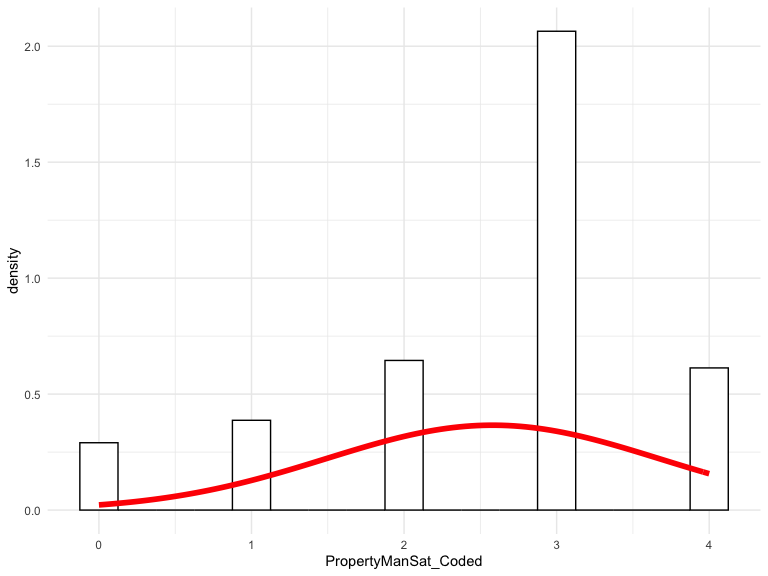
\includegraphics[width=0.9\linewidth]{Data-Cleaning-Coding_files/figure-latex/unnamed-chunk-12-1}

\hypertarget{independent-variables}{%
\paragraph{Independent Variables}\label{independent-variables}}

\begin{Shaded}
\begin{Highlighting}[]
\NormalTok{CodedData_VariablesofInterest }\OperatorTok\StringTok{ }
\StringTok{  }\KeywordTok{group_by}\NormalTok{(Smoke) }\OperatorTok\StringTok{ }
\StringTok{  }\KeywordTok{summarize}\NormalTok{(}\DataTypeTok{n=}\KeywordTok{n}\NormalTok{()) }\OperatorTok\StringTok{ }
\StringTok{  }\KeywordTok{mutate}\NormalTok{(}
    \DataTypeTok{percent =}\NormalTok{ n}\OperatorTok{/}\DecValTok{124}\OperatorTok{*}\DecValTok{100}\NormalTok{) }\OperatorTok\StringTok{ }
\StringTok{  }\KeywordTok{mutate}\NormalTok{(}
    \DataTypeTok{Smoke =} \KeywordTok{recode}\NormalTok{(Smoke,}
                   \StringTok{"0"}\NormalTok{ =}\StringTok{ "Non-smoker(s)"}\NormalTok{,}
                   \StringTok{"1"}\NormalTok{ =}\StringTok{ "Smoker(s)"}\NormalTok{)) }\OperatorTok\StringTok{ }
\StringTok{  }\NormalTok{knitr}\OperatorTok{::}\KeywordTok{kable}\NormalTok{(}\DataTypeTok{col.names=}\KeywordTok{c}\NormalTok{(}\StringTok{"Smoking Status"}\NormalTok{, }\StringTok{"n"}\NormalTok{, }\StringTok{"Percent(%)"}\NormalTok{), }\DataTypeTok{digits =} \DecValTok{2}\NormalTok{)}
\end{Highlighting}
\end{Shaded}

\begin{longtable}[]{@{}lrr@{}}
\toprule
Smoking Status & n & Percent(\%)\tabularnewline
\midrule
\endhead
Non-smoker(s) & 97 & 78.23\tabularnewline
Smoker(s) & 27 & 21.77\tabularnewline
\bottomrule
\end{longtable}

\begin{Shaded}
\begin{Highlighting}[]
\NormalTok{CodedData_VariablesofInterest }\OperatorTok\StringTok{ }
\StringTok{  }\KeywordTok{group_by}\NormalTok{(Race) }\OperatorTok\StringTok{ }
\StringTok{  }\KeywordTok{summarize}\NormalTok{(}\DataTypeTok{n=}\KeywordTok{n}\NormalTok{()) }\OperatorTok
\StringTok{   }\KeywordTok{mutate}\NormalTok{(}
  \DataTypeTok{percent =}\NormalTok{ n}\OperatorTok{/}\DecValTok{124}\OperatorTok{*}\DecValTok{100}\NormalTok{) }\OperatorTok\StringTok{ }
\StringTok{  }\KeywordTok{mutate}\NormalTok{(}
    \DataTypeTok{Race =} \KeywordTok{recode}\NormalTok{(Race,}
                  \StringTok{"Other, specify:"}\NormalTok{ =}\StringTok{ "Other"}\NormalTok{)}
\NormalTok{  ) }\OperatorTok\StringTok{ }
\StringTok{  }\NormalTok{knitr}\OperatorTok{::}\KeywordTok{kable}\NormalTok{(}\DataTypeTok{col.names=}\KeywordTok{c}\NormalTok{(}\StringTok{"Race/Ethnicity"}\NormalTok{, }\StringTok{"n"}\NormalTok{, }\StringTok{"Percent(%)"}\NormalTok{), }\DataTypeTok{digits =} \DecValTok{2}\NormalTok{)}
\end{Highlighting}
\end{Shaded}

\begin{longtable}[]{@{}lrr@{}}
\toprule
Race/Ethnicity & n & Percent(\%)\tabularnewline
\midrule
\endhead
Bi/Multiracial & 5 & 4.03\tabularnewline
Hispanic or Latinx & 87 & 70.16\tabularnewline
Non- Hispanic Black or African American & 26 & 20.97\tabularnewline
Other & 6 & 4.84\tabularnewline
\bottomrule
\end{longtable}

\begin{Shaded}
\begin{Highlighting}[]
\NormalTok{CodedData_VariablesofInterest }\OperatorTok\StringTok{ }
\StringTok{  }\KeywordTok{group_by}\NormalTok{(Age_Category) }\OperatorTok\StringTok{ }
\StringTok{  }\KeywordTok{summarize}\NormalTok{(}\DataTypeTok{n=}\KeywordTok{n}\NormalTok{()) }\OperatorTok
\StringTok{  }\KeywordTok{mutate}\NormalTok{(}
  \DataTypeTok{percent =}\NormalTok{ n}\OperatorTok{/}\DecValTok{124}\OperatorTok{*}\DecValTok{100}\NormalTok{) }\OperatorTok\StringTok{ }
\StringTok{  }\NormalTok{knitr}\OperatorTok{::}\KeywordTok{kable}\NormalTok{(}\DataTypeTok{col.names=}\KeywordTok{c}\NormalTok{(}\StringTok{"Age Group"}\NormalTok{, }\StringTok{"n"}\NormalTok{, }\StringTok{"Percent(%)"}\NormalTok{), }\DataTypeTok{digits =} \DecValTok{2}\NormalTok{)}
\end{Highlighting}
\end{Shaded}

\begin{longtable}[]{@{}lrr@{}}
\toprule
Age Group & n & Percent(\%)\tabularnewline
\midrule
\endhead
18-24 & 7 & 5.65\tabularnewline
25-44 & 25 & 20.16\tabularnewline
45-64 & 47 & 37.90\tabularnewline
65+ & 43 & 34.68\tabularnewline
NA & 2 & 1.61\tabularnewline
\bottomrule
\end{longtable}

\begin{Shaded}
\begin{Highlighting}[]
\NormalTok{CodedData_VariablesofInterest }\OperatorTok\StringTok{ }
\StringTok{  }\KeywordTok{drop_na}\NormalTok{() }\OperatorTok\StringTok{ }
\StringTok{  }\KeywordTok{group_by}\NormalTok{(Age, Gender) }\OperatorTok\StringTok{ }
\StringTok{  }\KeywordTok{ggplot}\NormalTok{(}\KeywordTok{aes}\NormalTok{(}\DataTypeTok{x=}\NormalTok{Gender, }\DataTypeTok{y=}\NormalTok{Age)) }\OperatorTok{+}\StringTok{ }\KeywordTok{geom_violin}\NormalTok{() }\OperatorTok{+}
\StringTok{  }\KeywordTok{labs}\NormalTok{(}\DataTypeTok{x =} \StringTok{"Gender"}\NormalTok{,}
      \DataTypeTok{y =} \StringTok{"Age"}\NormalTok{,}
      \DataTypeTok{title =} \StringTok{"Figure 1. Distribution of Age by Gender"}\NormalTok{)}
\end{Highlighting}
\end{Shaded}

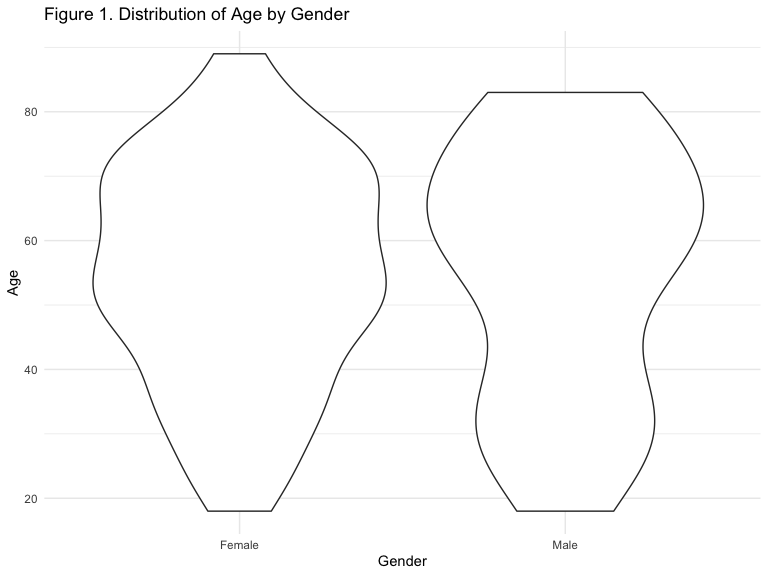
\includegraphics[width=0.9\linewidth]{Data-Cleaning-Coding_files/figure-latex/unnamed-chunk-16-1}

\begin{Shaded}
\begin{Highlighting}[]
\NormalTok{CodedData_VariablesofInterest }\OperatorTok\StringTok{ }
\StringTok{  }\KeywordTok{group_by}\NormalTok{(Gender) }\OperatorTok\StringTok{ }
\StringTok{  }\KeywordTok{summarize}\NormalTok{(}\DataTypeTok{n=}\KeywordTok{n}\NormalTok{()) }\OperatorTok
\StringTok{  }\KeywordTok{mutate}\NormalTok{(}
  \DataTypeTok{percent =}\NormalTok{ n}\OperatorTok{/}\DecValTok{124}\OperatorTok{*}\DecValTok{100}\NormalTok{) }\OperatorTok\StringTok{ }
\StringTok{  }\NormalTok{knitr}\OperatorTok{::}\KeywordTok{kable}\NormalTok{(}\DataTypeTok{col.names=}\KeywordTok{c}\NormalTok{(}\StringTok{"Gender"}\NormalTok{, }\StringTok{"n"}\NormalTok{, }\StringTok{"Percent(%)"}\NormalTok{), }\DataTypeTok{digits =} \DecValTok{2}\NormalTok{)}
\end{Highlighting}
\end{Shaded}

\begin{longtable}[]{@{}lrr@{}}
\toprule
Gender & n & Percent(\%)\tabularnewline
\midrule
\endhead
Female & 97 & 78.23\tabularnewline
Male & 26 & 20.97\tabularnewline
Other, please specify: & 1 & 0.81\tabularnewline
\bottomrule
\end{longtable}

\begin{Shaded}
\begin{Highlighting}[]
\NormalTok{CodedData_VariablesofInterest }\OperatorTok\StringTok{ }
\StringTok{  }\KeywordTok{drop_na}\NormalTok{() }\OperatorTok\StringTok{ }
\StringTok{  }\KeywordTok{select}\NormalTok{(Gender, Age) }\OperatorTok\StringTok{ }
\StringTok{  }\KeywordTok{group_by}\NormalTok{(Gender) }\OperatorTok\StringTok{ }
\StringTok{  }\KeywordTok{summarize}\NormalTok{(}\DataTypeTok{Mean =} \KeywordTok{mean}\NormalTok{(Age)) }\OperatorTok\StringTok{ }
\StringTok{  }\NormalTok{knitr}\OperatorTok{::}\KeywordTok{kable}\NormalTok{(}\DataTypeTok{col.names=}\KeywordTok{c}\NormalTok{(}\StringTok{"Age Group"}\NormalTok{, }\StringTok{"Mean Age"}\NormalTok{), }\DataTypeTok{digits =} \DecValTok{2}\NormalTok{)}
\end{Highlighting}
\end{Shaded}

\begin{longtable}[]{@{}lr@{}}
\toprule
Age Group & Mean Age\tabularnewline
\midrule
\endhead
Female & 54.76\tabularnewline
Male & 54.75\tabularnewline
\bottomrule
\end{longtable}

\begin{Shaded}
\begin{Highlighting}[]
\NormalTok{CodedData_VariablesofInterest }\OperatorTok\StringTok{ }
\StringTok{  }\KeywordTok{group_by}\NormalTok{(Income) }\OperatorTok\StringTok{ }
\StringTok{  }\KeywordTok{summarize}\NormalTok{(}\DataTypeTok{n=}\KeywordTok{n}\NormalTok{()) }\OperatorTok
\StringTok{  }\KeywordTok{mutate}\NormalTok{(}
  \DataTypeTok{percent =}\NormalTok{ n}\OperatorTok{/}\DecValTok{124}\OperatorTok{*}\DecValTok{100}\NormalTok{) }\OperatorTok\StringTok{ }
\StringTok{  }\NormalTok{knitr}\OperatorTok{::}\KeywordTok{kable}\NormalTok{(}\DataTypeTok{col.names=}\KeywordTok{c}\NormalTok{(}\StringTok{"Income Category"}\NormalTok{, }\StringTok{"n"}\NormalTok{, }\StringTok{"Percent(%)"}\NormalTok{), }\DataTypeTok{digits =} \DecValTok{2}\NormalTok{)}
\end{Highlighting}
\end{Shaded}

\begin{longtable}[]{@{}rrr@{}}
\toprule
Income Category & n & Percent(\%)\tabularnewline
\midrule
\endhead
1 & 16 & 12.90\tabularnewline
2 & 9 & 7.26\tabularnewline
3 & 28 & 22.58\tabularnewline
4 & 24 & 19.35\tabularnewline
5 & 29 & 23.39\tabularnewline
6 & 3 & 2.42\tabularnewline
7 & 5 & 4.03\tabularnewline
8 & 3 & 2.42\tabularnewline
9 & 2 & 1.61\tabularnewline
10 & 2 & 1.61\tabularnewline
NA & 3 & 2.42\tabularnewline
\bottomrule
\end{longtable}

\begin{Shaded}
\begin{Highlighting}[]
\NormalTok{CodedData_VariablesofInterest }\OperatorTok\StringTok{ }
\StringTok{  }\KeywordTok{group_by}\NormalTok{(Education) }\OperatorTok\StringTok{ }
\StringTok{  }\KeywordTok{summarize}\NormalTok{(}\DataTypeTok{n=}\KeywordTok{n}\NormalTok{()) }\OperatorTok
\StringTok{  }\KeywordTok{mutate}\NormalTok{(}
  \DataTypeTok{percent =}\NormalTok{ n}\OperatorTok{/}\DecValTok{124}\OperatorTok{*}\DecValTok{100}\NormalTok{) }\OperatorTok\StringTok{ }
\StringTok{  }\NormalTok{knitr}\OperatorTok{::}\KeywordTok{kable}\NormalTok{(}\DataTypeTok{col.names=}\KeywordTok{c}\NormalTok{(}\StringTok{"Education Completed"}\NormalTok{, }\StringTok{"n"}\NormalTok{, }\StringTok{"Percent(%)"}\NormalTok{), }\DataTypeTok{digits =} \DecValTok{2}\NormalTok{)}
\end{Highlighting}
\end{Shaded}

\begin{longtable}[]{@{}lrr@{}}
\toprule
Education Completed & n & Percent(\%)\tabularnewline
\midrule
\endhead
2 Year Community College Degree & 7 & 5.65\tabularnewline
4 Year College Degree & 6 & 4.84\tabularnewline
G.E.D. & 5 & 4.03\tabularnewline
High School/Secondary School Diploma & 41 & 33.06\tabularnewline
Less than High School & 53 & 42.74\tabularnewline
Other, please specify: & 4 & 3.23\tabularnewline
Post-Graduate Degree & 3 & 2.42\tabularnewline
Some College & 2 & 1.61\tabularnewline
Vocational School & 3 & 2.42\tabularnewline
\bottomrule
\end{longtable}

\hypertarget{x2-tables-and-visualizations}{%
\subsubsection{2x2 Tables and
Visualizations}\label{x2-tables-and-visualizations}}

\begin{Shaded}
\begin{Highlighting}[]
\NormalTok{CodedData_VariablesofInterest }\OperatorTok\StringTok{ }
\StringTok{  }\KeywordTok{group_by}\NormalTok{(Age_Category, Gender) }\OperatorTok\StringTok{ }
\StringTok{  }\KeywordTok{summarize}\NormalTok{(}\DataTypeTok{n=}\KeywordTok{n}\NormalTok{()) }\OperatorTok
\StringTok{  }\KeywordTok{pivot_wider}\NormalTok{(}
    \DataTypeTok{names_from =}\NormalTok{ Gender,}
    \DataTypeTok{values_from =}\NormalTok{ n) }\OperatorTok\StringTok{ }
\StringTok{  }\NormalTok{knitr}\OperatorTok{::}\KeywordTok{kable}\NormalTok{(}\DataTypeTok{col.names =} \KeywordTok{c}\NormalTok{(}\StringTok{"Age Group"}\NormalTok{,}\StringTok{"Female (n)"}\NormalTok{, }\StringTok{"Male (n)"}\NormalTok{, }\StringTok{"Other (n)"}\NormalTok{))}
\end{Highlighting}
\end{Shaded}

\begin{longtable}[]{@{}lrrr@{}}
\toprule
Age Group & Female (n) & Male (n) & Other (n)\tabularnewline
\midrule
\endhead
18-24 & 5 & 2 & NA\tabularnewline
25-44 & 19 & 6 & NA\tabularnewline
45-64 & 38 & 8 & 1\tabularnewline
65+ & 33 & 10 & NA\tabularnewline
NA & 2 & NA & NA\tabularnewline
\bottomrule
\end{longtable}

\begin{Shaded}
\begin{Highlighting}[]
\NormalTok{CodedData_VariablesofInterest }\OperatorTok\StringTok{ }
\StringTok{  }\KeywordTok{drop_na}\NormalTok{() }\OperatorTok\StringTok{ }
\StringTok{  }\KeywordTok{select}\NormalTok{(Income, Age_Category) }\OperatorTok\StringTok{ }
\StringTok{  }\KeywordTok{group_by}\NormalTok{(Age_Category) }\OperatorTok\StringTok{ }
\StringTok{  }\KeywordTok{summarize}\NormalTok{(}\DataTypeTok{Mean =} \KeywordTok{mean}\NormalTok{(Income)) }\OperatorTok\StringTok{ }
\StringTok{  }\NormalTok{knitr}\OperatorTok{::}\KeywordTok{kable}\NormalTok{(}\DataTypeTok{col.names=}\KeywordTok{c}\NormalTok{(}\StringTok{"Age Group"}\NormalTok{, }\StringTok{"Mean Income"}\NormalTok{),}\DataTypeTok{digits =} \DecValTok{2}\NormalTok{)}
\end{Highlighting}
\end{Shaded}

\begin{longtable}[]{@{}lr@{}}
\toprule
Age Group & Mean Income\tabularnewline
\midrule
\endhead
18-24 & 5.00\tabularnewline
25-44 & 3.96\tabularnewline
45-64 & 3.91\tabularnewline
65+ & 3.87\tabularnewline
\bottomrule
\end{longtable}

\begin{Shaded}
\begin{Highlighting}[]
\NormalTok{CodedData_VariablesofInterest }\OperatorTok\StringTok{ }
\StringTok{  }\KeywordTok{ggplot}\NormalTok{(}\KeywordTok{aes}\NormalTok{(}\DataTypeTok{x=}\NormalTok{Age_Category, }\DataTypeTok{fill =}\NormalTok{ Gender)) }\OperatorTok{+}\StringTok{ }\KeywordTok{geom_bar}\NormalTok{() }\OperatorTok{+}
\StringTok{  }\KeywordTok{labs}\NormalTok{(}\DataTypeTok{x =} \StringTok{"Age Group"}\NormalTok{,}
      \DataTypeTok{y =} \StringTok{"Count"}\NormalTok{,}
      \DataTypeTok{color =} \StringTok{"Gender"}\NormalTok{,}
      \DataTypeTok{title =} \StringTok{"Figure 2. Age Group by Gender"}\NormalTok{)}
\end{Highlighting}
\end{Shaded}

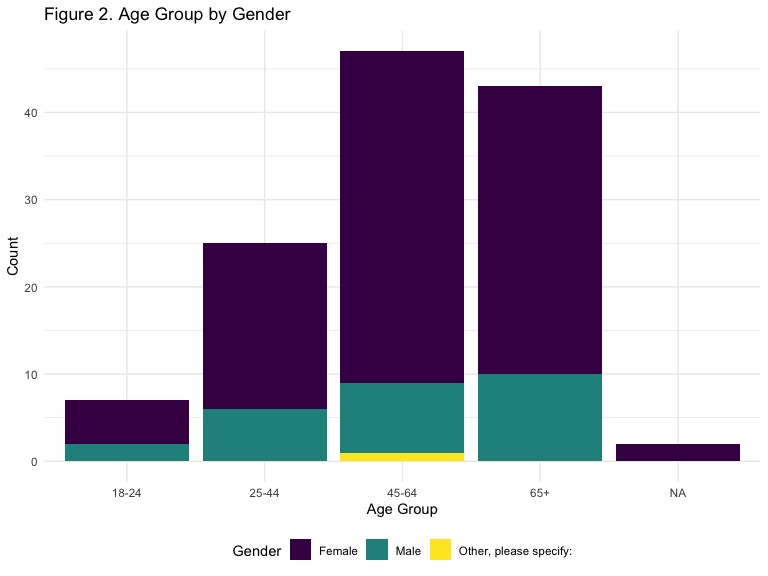
\includegraphics[width=0.9\linewidth]{Data-Cleaning-Coding_files/figure-latex/unnamed-chunk-23-1}

\begin{Shaded}
\begin{Highlighting}[]
\NormalTok{CodedData_VariablesofInterest }\OperatorTok
\StringTok{  }\KeywordTok{drop_na}\NormalTok{() }\OperatorTok\StringTok{ }
\StringTok{  }\KeywordTok{group_by}\NormalTok{(Age_Category, Race) }\OperatorTok\StringTok{ }
\StringTok{  }\KeywordTok{summarize}\NormalTok{(}\DataTypeTok{n=}\KeywordTok{n}\NormalTok{()) }\OperatorTok
\StringTok{  }\KeywordTok{pivot_wider}\NormalTok{(}
    \DataTypeTok{names_from =}\NormalTok{ Race,}
    \DataTypeTok{values_from =}\NormalTok{ n}
\NormalTok{  ) }\OperatorTok\StringTok{ }
\StringTok{  }\NormalTok{knitr}\OperatorTok{::}\KeywordTok{kable}\NormalTok{(}\DataTypeTok{col.names =} \KeywordTok{c}\NormalTok{(}\StringTok{"Age Group"}\NormalTok{, }\StringTok{"Hispanic or Latinx (n)"}\NormalTok{, }\StringTok{"Non-Hispanic Black or African American (n)"}\NormalTok{, }\StringTok{"Bi/Multiracial (n)"}\NormalTok{, }\StringTok{"Other (n)"}\NormalTok{))}
\end{Highlighting}
\end{Shaded}

\begin{longtable}[]{@{}lrrrr@{}}
\toprule
Age Group & Hispanic or Latinx (n) & Non-Hispanic Black or African
American (n) & Bi/Multiracial (n) & Other (n)\tabularnewline
\midrule
\endhead
18-24 & 5 & 2 & NA & NA\tabularnewline
25-44 & 14 & 7 & 3 & 1\tabularnewline
45-64 & 27 & 11 & 1 & 5\tabularnewline
65+ & 33 & 4 & 1 & NA\tabularnewline
\bottomrule
\end{longtable}

\begin{Shaded}
\begin{Highlighting}[]
\NormalTok{CodedData_VariablesofInterest }\OperatorTok\StringTok{ }
\StringTok{  }\KeywordTok{group_by}\NormalTok{(Age_Category, Race) }\OperatorTok\StringTok{ }
\StringTok{  }\KeywordTok{ggplot}\NormalTok{(}\KeywordTok{aes}\NormalTok{(}\DataTypeTok{x=}\NormalTok{ Age_Category, }\DataTypeTok{fill =}\NormalTok{ Race)) }\OperatorTok{+}\StringTok{ }\KeywordTok{geom_bar}\NormalTok{() }\OperatorTok{+}
\StringTok{  }\KeywordTok{labs}\NormalTok{(}\DataTypeTok{x =} \StringTok{"Age Group"}\NormalTok{,}
      \DataTypeTok{y =} \StringTok{"Count"}\NormalTok{,}
      \DataTypeTok{color =} \StringTok{"Race/Ethnicity"}\NormalTok{,}
      \DataTypeTok{title =} \StringTok{"Figure 3. Age by Race/Ethnicity"}\NormalTok{)}
\end{Highlighting}
\end{Shaded}

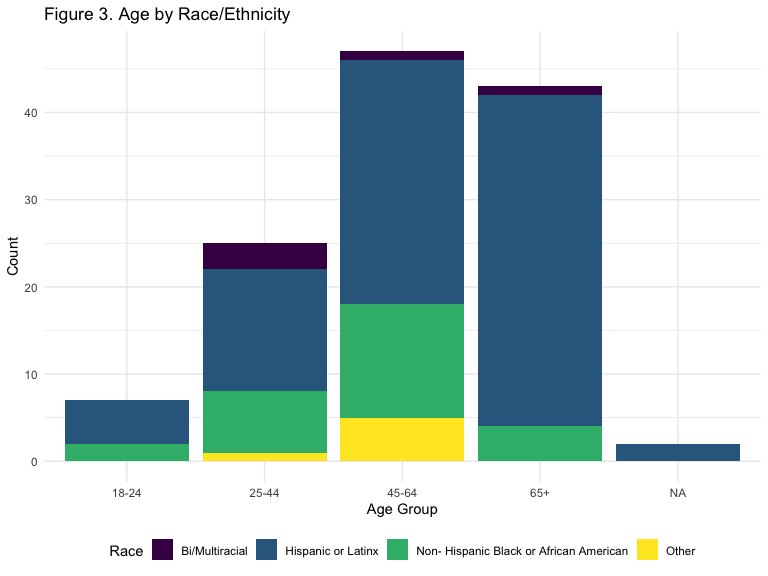
\includegraphics[width=0.9\linewidth]{Data-Cleaning-Coding_files/figure-latex/unnamed-chunk-25-1}

\begin{Shaded}
\begin{Highlighting}[]
\NormalTok{CodedData_VariablesofInterest }\OperatorTok
\StringTok{  }\KeywordTok{group_by}\NormalTok{(Race, Smoke) }\OperatorTok\StringTok{ }
\StringTok{  }\KeywordTok{summarize}\NormalTok{(}\DataTypeTok{n=}\KeywordTok{n}\NormalTok{()) }\OperatorTok
\StringTok{  }\KeywordTok{mutate}\NormalTok{(}
    \DataTypeTok{Smoke =} \KeywordTok{recode}\NormalTok{(Smoke,}
                   \StringTok{"0"}\NormalTok{ =}\StringTok{ "Non-smoker(s)"}\NormalTok{,}
                   \StringTok{"1"}\NormalTok{ =}\StringTok{ "Smoker(s)"}\NormalTok{)) }\OperatorTok\StringTok{ }
\StringTok{  }\KeywordTok{pivot_wider}\NormalTok{(}
    \DataTypeTok{names_from =}\NormalTok{ Race,}
    \DataTypeTok{values_from =}\NormalTok{ n) }\OperatorTok\StringTok{ }
\StringTok{  }\NormalTok{knitr}\OperatorTok{::}\KeywordTok{kable}\NormalTok{(}\DataTypeTok{col.names =} \KeywordTok{c}\NormalTok{(}\StringTok{"Smoking Status"}\NormalTok{, }\StringTok{"Bi/Multiracial (n)"}\NormalTok{, }\StringTok{"Hispanic or Latinx (n)"}\NormalTok{, }\StringTok{"Black or African American (n)"}\NormalTok{, }\StringTok{"Other (n)"}\NormalTok{))}
\end{Highlighting}
\end{Shaded}

\begin{longtable}[]{@{}lrrrr@{}}
\toprule
Smoking Status & Bi/Multiracial (n) & Hispanic or Latinx (n) & Black or
African American (n) & Other (n)\tabularnewline
\midrule
\endhead
Non-smoker(s) & 3 & 71 & 20 & 3\tabularnewline
Smoker(s) & 2 & 16 & 6 & 3\tabularnewline
\bottomrule
\end{longtable}

\begin{Shaded}
\begin{Highlighting}[]
\NormalTok{CodedData_VariablesofInterest }\OperatorTok
\StringTok{  }\KeywordTok{group_by}\NormalTok{(Age_Category, Smoke) }\OperatorTok\StringTok{ }
\StringTok{  }\KeywordTok{drop_na}\NormalTok{() }\OperatorTok\StringTok{ }
\StringTok{  }\KeywordTok{summarize}\NormalTok{(}\DataTypeTok{n=}\KeywordTok{n}\NormalTok{()) }\OperatorTok
\StringTok{  }\KeywordTok{mutate}\NormalTok{(}
    \DataTypeTok{Smoke =} \KeywordTok{recode}\NormalTok{(Smoke,}
                   \StringTok{"0"}\NormalTok{ =}\StringTok{ "Non-smoker(s)"}\NormalTok{,}
                   \StringTok{"1"}\NormalTok{ =}\StringTok{ "Smoker(s)"}\NormalTok{)) }\OperatorTok\StringTok{ }
\StringTok{  }\KeywordTok{pivot_wider}\NormalTok{(}
    \DataTypeTok{names_from =}\NormalTok{ Age_Category,}
    \DataTypeTok{values_from =}\NormalTok{ n) }\OperatorTok\StringTok{ }
\StringTok{  }\NormalTok{knitr}\OperatorTok{::}\KeywordTok{kable}\NormalTok{(}\DataTypeTok{col.names =} \KeywordTok{c}\NormalTok{(}\StringTok{"Smoking Status"}\NormalTok{, }\StringTok{"18-24 (n)"}\NormalTok{, }\StringTok{"25-44 (n)"}\NormalTok{, }\StringTok{"45-64 (n)"}\NormalTok{, }\StringTok{"65+ (n)"}\NormalTok{))}
\end{Highlighting}
\end{Shaded}

\begin{longtable}[]{@{}lrrrr@{}}
\toprule
Smoking Status & 18-24 (n) & 25-44 (n) & 45-64 (n) & 65+
(n)\tabularnewline
\midrule
\endhead
Non-smoker(s) & 6 & 16 & 34 & 33\tabularnewline
Smoker(s) & 1 & 9 & 10 & 5\tabularnewline
\bottomrule
\end{longtable}

\begin{Shaded}
\begin{Highlighting}[]
\NormalTok{CodedData_VariablesofInterest }\OperatorTok\StringTok{ }
\StringTok{  }\KeywordTok{mutate}\NormalTok{(}
    \DataTypeTok{Smoke =} \KeywordTok{recode}\NormalTok{(Smoke,}
                   \StringTok{"0"}\NormalTok{ =}\StringTok{ "Non-smoker(s)"}\NormalTok{,}
                   \StringTok{"1"}\NormalTok{ =}\StringTok{ "Smoker(s)"}\NormalTok{)}
\NormalTok{  ) }\OperatorTok\StringTok{ }
\KeywordTok{ggplot}\NormalTok{(}\KeywordTok{aes}\NormalTok{(}\DataTypeTok{x=}\NormalTok{Smoke, }\DataTypeTok{y=}\NormalTok{Age)) }\OperatorTok{+}\StringTok{ }
\StringTok{  }\KeywordTok{geom_boxplot}\NormalTok{(}\DataTypeTok{outlier.shape=}\OtherTok{NA}\NormalTok{) }\OperatorTok{+}\StringTok{ }\CommentTok{#avoid plotting outliers twice}
\StringTok{  }\KeywordTok{geom_jitter}\NormalTok{(}\DataTypeTok{position=}\KeywordTok{position_jitter}\NormalTok{(}\DataTypeTok{width=}\NormalTok{.}\DecValTok{1}\NormalTok{, }\DataTypeTok{height=}\DecValTok{0}\NormalTok{)) }\OperatorTok{+}\StringTok{ }
\StringTok{  }\KeywordTok{labs}\NormalTok{(}\DataTypeTok{x =} \StringTok{"Smoking Status"}\NormalTok{,}
      \DataTypeTok{y =} \StringTok{"Age"}\NormalTok{,}
      \DataTypeTok{title =} \StringTok{"Figure 4. Distribution of Age by Smoking Status"}\NormalTok{)}
\end{Highlighting}
\end{Shaded}

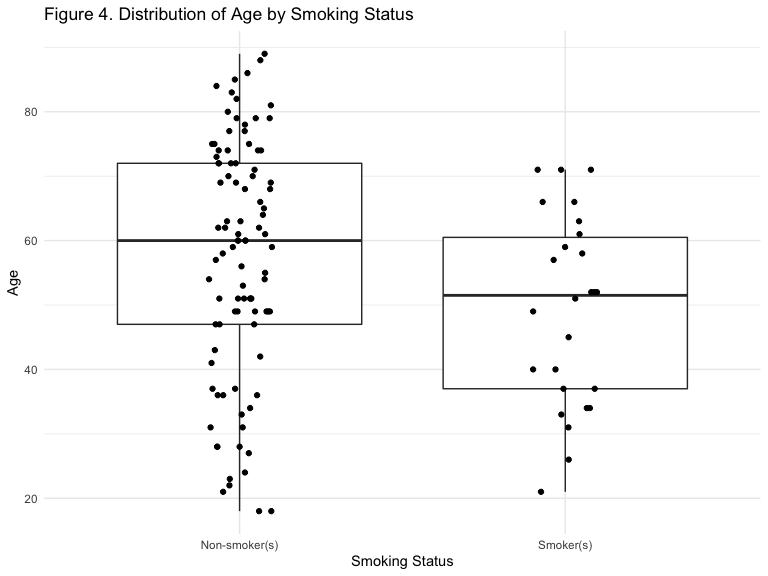
\includegraphics[width=0.9\linewidth]{Data-Cleaning-Coding_files/figure-latex/unnamed-chunk-28-1}

\begin{Shaded}
\begin{Highlighting}[]
\NormalTok{CodedData_VariablesofInterest }\OperatorTok\StringTok{ }
\StringTok{  }\KeywordTok{group_by}\NormalTok{(Age_Category, Education) }\OperatorTok\StringTok{ }
\StringTok{  }\KeywordTok{drop_na}\NormalTok{() }\OperatorTok\StringTok{ }
\StringTok{  }\KeywordTok{ggplot}\NormalTok{(}\KeywordTok{aes}\NormalTok{(}\DataTypeTok{x=}\NormalTok{ Age_Category, }\DataTypeTok{fill =}\NormalTok{ Education)) }\OperatorTok{+}\StringTok{ }\KeywordTok{geom_bar}\NormalTok{() }\OperatorTok{+}\StringTok{ }\KeywordTok{coord_flip}\NormalTok{() }\OperatorTok{+}
\StringTok{  }\KeywordTok{labs}\NormalTok{(}\DataTypeTok{x =} \StringTok{"Age Group"}\NormalTok{,}
      \DataTypeTok{y =} \StringTok{"Count"}\NormalTok{,}
      \DataTypeTok{color =} \StringTok{"Education"}\NormalTok{,}
      \DataTypeTok{title =} \StringTok{"Figure 5. Education by Age Group"}\NormalTok{) }\OperatorTok{+}
\KeywordTok{theme}\NormalTok{(}\DataTypeTok{legend.position =} \StringTok{"bottom"}\NormalTok{)}
\end{Highlighting}
\end{Shaded}

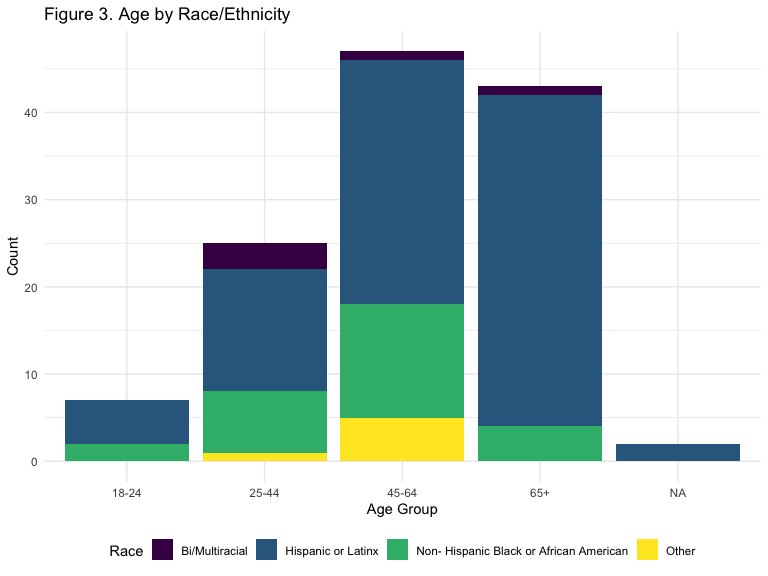
\includegraphics[width=0.9\linewidth]{Data-Cleaning-Coding_files/figure-latex/unnamed-chunk-29-1}

\hypertarget{exploratory-analyses-of-relationships-between-variables}{%
\subsubsection{Exploratory Analyses of Relationships between
Variables}\label{exploratory-analyses-of-relationships-between-variables}}

\begin{Shaded}
\begin{Highlighting}[]
\CommentTok{#Part 1}
\NormalTok{CodedData_VariablesofInterest }\OperatorTok\StringTok{  }
\StringTok{  }\KeywordTok{group_by}\NormalTok{(total_PSS_score, composite_sf36_score, Age_Category) }\OperatorTok
\StringTok{  }\KeywordTok{summarize}\NormalTok{(}\DataTypeTok{n=}\KeywordTok{n}\NormalTok{()) }\OperatorTok\StringTok{ }
\StringTok{  }\KeywordTok{ggplot}\NormalTok{(}\KeywordTok{aes}\NormalTok{(}\DataTypeTok{x =}\NormalTok{ total_PSS_score, }\DataTypeTok{y =}\NormalTok{ composite_sf36_score,  }\DataTypeTok{color =}\NormalTok{ Age_Category)) }\OperatorTok{+}
\StringTok{  }\KeywordTok{geom_point}\NormalTok{(}\DataTypeTok{size =} \FloatTok{1.5}\NormalTok{, }\DataTypeTok{alpha =} \FloatTok{0.8}\NormalTok{) }\OperatorTok{+}
\StringTok{  }\KeywordTok{geom_smooth}\NormalTok{(}\DataTypeTok{method =}\NormalTok{lm, }\DataTypeTok{color =} \StringTok{"black"}\NormalTok{, }\DataTypeTok{linetype =} \DecValTok{1}\NormalTok{) }\OperatorTok{+}
\StringTok{  }\KeywordTok{labs}\NormalTok{(}
      \DataTypeTok{x =} \StringTok{"Perceived Stress Score"}\NormalTok{,}
      \DataTypeTok{y =} \StringTok{"Overall Health Score"}\NormalTok{,}
      \DataTypeTok{color =} \StringTok{"Age"}\NormalTok{,}
      \DataTypeTok{title =} \StringTok{"Figure 6. Relationship between Perceived Stress and Health Status"}\NormalTok{) }\OperatorTok{+}
\StringTok{      }\KeywordTok{theme}\NormalTok{(}\DataTypeTok{legend.position =} \StringTok{"right"}\NormalTok{) }
\end{Highlighting}
\end{Shaded}

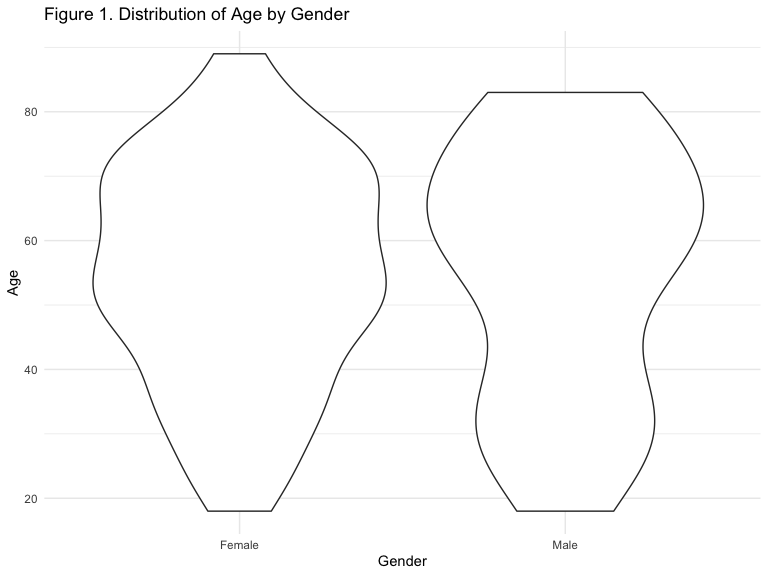
\includegraphics[width=0.9\linewidth]{Data-Cleaning-Coding_files/figure-latex/unnamed-chunk-30-1}

\begin{Shaded}
\begin{Highlighting}[]
\CommentTok{#Part 2}
\NormalTok{CodedData_VariablesofInterest }\OperatorTok\StringTok{  }
\StringTok{  }\KeywordTok{group_by}\NormalTok{(HousingSatisfactionScore, composite_sf36_score, Age_Category) }\OperatorTok
\StringTok{  }\KeywordTok{summarize}\NormalTok{(}\DataTypeTok{n=}\KeywordTok{n}\NormalTok{()) }\OperatorTok\StringTok{ }
\StringTok{  }\KeywordTok{ggplot}\NormalTok{(}\KeywordTok{aes}\NormalTok{(}\DataTypeTok{x =}\NormalTok{ HousingSatisfactionScore, }\DataTypeTok{y =}\NormalTok{ composite_sf36_score,  }\DataTypeTok{color =}\NormalTok{ Age_Category)) }\OperatorTok{+}
\StringTok{  }\KeywordTok{geom_point}\NormalTok{(}\DataTypeTok{size =} \DecValTok{1}\NormalTok{, }\DataTypeTok{alpha =} \FloatTok{0.5}\NormalTok{) }\OperatorTok{+}
\StringTok{  }\KeywordTok{geom_smooth}\NormalTok{(}\DataTypeTok{method =}\NormalTok{lm, }\DataTypeTok{color =} \StringTok{"black"}\NormalTok{, }\DataTypeTok{linetype =} \DecValTok{1}\NormalTok{) }\OperatorTok{+}
\StringTok{  }\KeywordTok{labs}\NormalTok{(}
      \DataTypeTok{x =} \StringTok{"Housing Satisfaction Score"}\NormalTok{,}
      \DataTypeTok{y =} \StringTok{"Overall Health Score"}\NormalTok{,}
      \DataTypeTok{color =} \StringTok{"Age"}\NormalTok{,}
      \DataTypeTok{title =} \StringTok{"Figure 7. Relationship between Housing Satisfaction and Health Status"}\NormalTok{) }\OperatorTok{+}
\StringTok{      }\KeywordTok{theme}\NormalTok{(}\DataTypeTok{legend.position =} \StringTok{"right"}\NormalTok{)}
\end{Highlighting}
\end{Shaded}

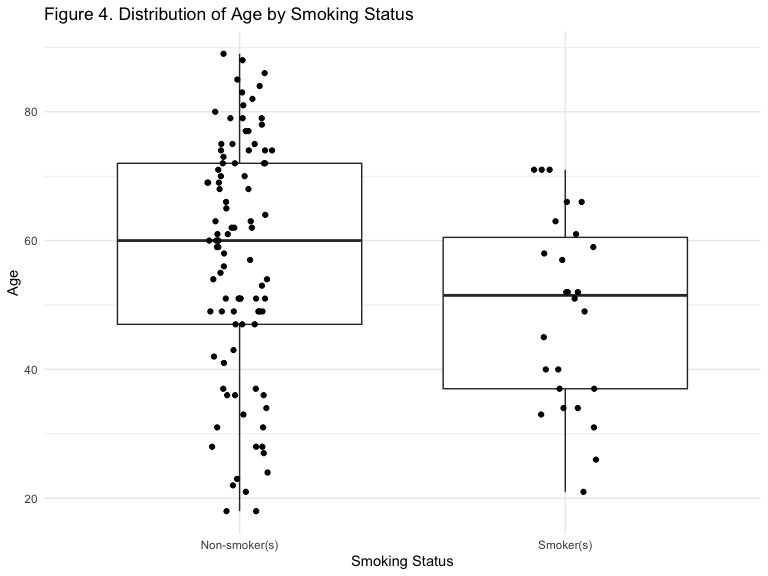
\includegraphics[width=0.9\linewidth]{Data-Cleaning-Coding_files/figure-latex/unnamed-chunk-31-1}

\begin{Shaded}
\begin{Highlighting}[]
\CommentTok{#Part 3}
\NormalTok{CodedData_VariablesofInterest }\OperatorTok\StringTok{  }
\StringTok{  }\KeywordTok{group_by}\NormalTok{(HousingSatisfactionScore, total_PSS_score, Age_Category) }\OperatorTok
\StringTok{  }\KeywordTok{summarize}\NormalTok{(}\DataTypeTok{n=}\KeywordTok{n}\NormalTok{()) }\OperatorTok\StringTok{ }
\StringTok{  }\KeywordTok{ggplot}\NormalTok{(}\KeywordTok{aes}\NormalTok{(}\DataTypeTok{x =}\NormalTok{ HousingSatisfactionScore, }\DataTypeTok{y =}\NormalTok{ total_PSS_score,  }\DataTypeTok{color =}\NormalTok{ Age_Category)) }\OperatorTok{+}
\StringTok{  }\KeywordTok{geom_point}\NormalTok{(}\DataTypeTok{size =} \FloatTok{1.5}\NormalTok{, }\DataTypeTok{alpha =} \FloatTok{0.8}\NormalTok{) }\OperatorTok{+}
\StringTok{  }\KeywordTok{geom_smooth}\NormalTok{(}\DataTypeTok{method =}\NormalTok{lm, }\DataTypeTok{color =} \StringTok{"black"}\NormalTok{, }\DataTypeTok{linetype =} \DecValTok{1}\NormalTok{) }\OperatorTok{+}
\StringTok{  }\KeywordTok{labs}\NormalTok{(}
      \DataTypeTok{x =} \StringTok{"Housing Satisfaction Score"}\NormalTok{,}
      \DataTypeTok{y =} \StringTok{"Perceived Stress Score"}\NormalTok{,}
      \DataTypeTok{color =} \StringTok{"Age"}\NormalTok{,}
      \DataTypeTok{title =} \StringTok{"Figure 8. Relationship between Housing Satisfaction and Perceived Stress"}\NormalTok{) }\OperatorTok{+}
\StringTok{      }\KeywordTok{theme}\NormalTok{(}\DataTypeTok{legend.position =} \StringTok{"right"}\NormalTok{)}
\end{Highlighting}
\end{Shaded}

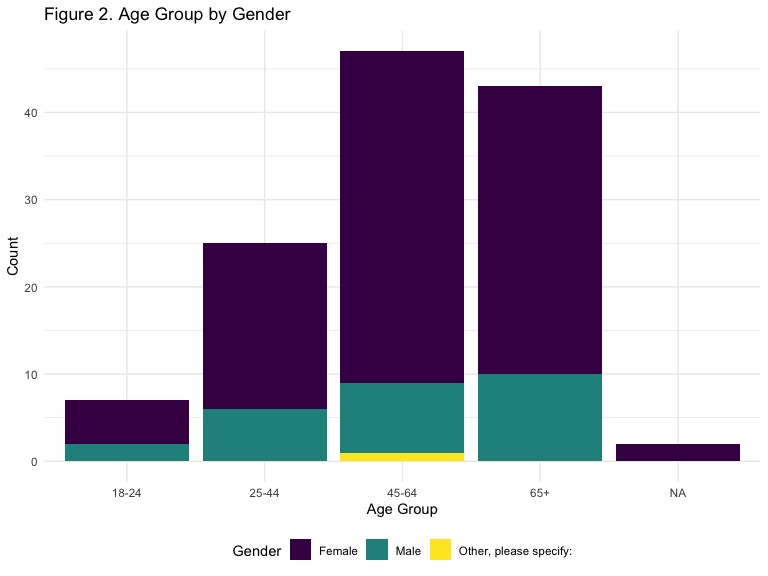
\includegraphics[width=0.9\linewidth]{Data-Cleaning-Coding_files/figure-latex/unnamed-chunk-32-1}

\hypertarget{initial-bivariate-analyses}{%
\subsubsection{Initial bivariate
analyses}\label{initial-bivariate-analyses}}

\hypertarget{bivariate-model-1-composite_sf36_score-b_0-b_1-total_pss_score_i}{%
\subparagraph{Bivariate model 1 : composite\_sf36\_score
\textasciitilde{} b\_0 + b\_1
total\_PSS\_score\_i}\label{bivariate-model-1-composite_sf36_score-b_0-b_1-total_pss_score_i}}

\begin{Shaded}
\begin{Highlighting}[]
\NormalTok{bivariate1 =}\StringTok{ }\KeywordTok{lm}\NormalTok{(composite_sf36_score }\OperatorTok{~}\StringTok{ }\NormalTok{total_PSS_score, }\DataTypeTok{data =}\NormalTok{ CodedData_VariablesofInterest)}
\KeywordTok{summary}\NormalTok{(bivariate1) }
\end{Highlighting}
\end{Shaded}

\begin{verbatim}
## 
## Call:
## lm(formula = composite_sf36_score ~ total_PSS_score, data = CodedData_VariablesofInterest)
## 
## Residuals:
##     Min      1Q  Median      3Q     Max 
## -52.225 -14.892   2.345  17.752  45.795 
## 
## Coefficients:
##                 Estimate Std. Error t value Pr(>|t|)    
## (Intercept)      88.1490     3.8970  22.620  < 2e-16 ***
## total_PSS_score  -3.3462     0.4593  -7.286 3.92e-11 ***
## ---
## Signif. codes:  0 '***' 0.001 '**' 0.01 '*' 0.05 '.' 0.1 ' ' 1
## 
## Residual standard error: 22.25 on 118 degrees of freedom
##   (4 observations deleted due to missingness)
## Multiple R-squared:  0.3103, Adjusted R-squared:  0.3044 
## F-statistic: 53.08 on 1 and 118 DF,  p-value: 3.924e-11
\end{verbatim}

\begin{Shaded}
\begin{Highlighting}[]
\NormalTok{bivariate1 }\OperatorTok\StringTok{ }
\StringTok{  }\NormalTok{broom}\OperatorTok{::}\KeywordTok{tidy}\NormalTok{() }\OperatorTok\StringTok{ }
\StringTok{  }\KeywordTok{mutate}\NormalTok{(}
         \DataTypeTok{High_CI =} \KeywordTok{exp}\NormalTok{(estimate }\OperatorTok{+}\StringTok{ }\FloatTok{1.96}\OperatorTok{*}\NormalTok{std.error),}
         \DataTypeTok{Low_CI =} \KeywordTok{exp}\NormalTok{(estimate }\OperatorTok{-}\StringTok{ }\FloatTok{1.96}\OperatorTok{*}\NormalTok{std.error)) }\OperatorTok\StringTok{ }
\StringTok{  }\KeywordTok{select}\NormalTok{(term, estimate, p.value, Low_CI, High_CI) }\OperatorTok\StringTok{ }
\StringTok{  }\NormalTok{knitr}\OperatorTok{::}\KeywordTok{kable}\NormalTok{(}\DataTypeTok{digits =} \DecValTok{3}\NormalTok{)}
\end{Highlighting}
\end{Shaded}

\begin{longtable}[]{@{}lrrrr@{}}
\toprule
term & estimate & p.value & Low\_CI & High\_CI\tabularnewline
\midrule
\endhead
(Intercept) & 88.149 & 0 & 9.234996e+34 & 3.979489e+41\tabularnewline
total\_PSS\_score & -3.346 & 0 & 1.400000e-02 &
8.700000e-02\tabularnewline
\bottomrule
\end{longtable}

\hypertarget{bivariate-model-2-composite_sf36_score-b_0-b_1-age_i}{%
\subparagraph{Bivariate model 2 : composite\_sf36\_score
\textasciitilde{} b\_0 + b\_1
Age\_i}\label{bivariate-model-2-composite_sf36_score-b_0-b_1-age_i}}

\begin{Shaded}
\begin{Highlighting}[]
\NormalTok{bivariate2 =}\StringTok{ }\KeywordTok{lm}\NormalTok{(composite_sf36_score }\OperatorTok{~}\StringTok{ }\NormalTok{Age, }\DataTypeTok{data =}\NormalTok{ CodedData_VariablesofInterest)}
\KeywordTok{summary}\NormalTok{(bivariate2)}
\end{Highlighting}
\end{Shaded}

\begin{verbatim}
## 
## Call:
## lm(formula = composite_sf36_score ~ Age, data = CodedData_VariablesofInterest)
## 
## Residuals:
##     Min      1Q  Median      3Q     Max 
## -68.622 -17.200   1.028  20.986  43.485 
## 
## Coefficients:
##             Estimate Std. Error t value Pr(>|t|)    
## (Intercept)  86.5376     7.6771  11.272  < 2e-16 ***
## Age          -0.4289     0.1321  -3.246  0.00152 ** 
## ---
## Signif. codes:  0 '***' 0.001 '**' 0.01 '*' 0.05 '.' 0.1 ' ' 1
## 
## Residual standard error: 25.61 on 118 degrees of freedom
##   (4 observations deleted due to missingness)
## Multiple R-squared:  0.08197,    Adjusted R-squared:  0.07419 
## F-statistic: 10.54 on 1 and 118 DF,  p-value: 0.001524
\end{verbatim}

\begin{Shaded}
\begin{Highlighting}[]
\NormalTok{bivariate2 }\OperatorTok\StringTok{ }
\StringTok{  }\NormalTok{broom}\OperatorTok{::}\KeywordTok{tidy}\NormalTok{() }\OperatorTok\StringTok{ }
\StringTok{  }\KeywordTok{mutate}\NormalTok{(}
         \DataTypeTok{High_CI =} \KeywordTok{exp}\NormalTok{(estimate }\OperatorTok{+}\StringTok{ }\FloatTok{1.96}\OperatorTok{*}\NormalTok{std.error),}
         \DataTypeTok{Low_CI =} \KeywordTok{exp}\NormalTok{(estimate }\OperatorTok{-}\StringTok{ }\FloatTok{1.96}\OperatorTok{*}\NormalTok{std.error)) }\OperatorTok\StringTok{ }
\StringTok{  }\KeywordTok{select}\NormalTok{(term, estimate, p.value, Low_CI, High_CI) }\OperatorTok\StringTok{ }
\StringTok{  }\NormalTok{knitr}\OperatorTok{::}\KeywordTok{kable}\NormalTok{(}\DataTypeTok{digits =} \DecValTok{3}\NormalTok{)}
\end{Highlighting}
\end{Shaded}

\begin{longtable}[]{@{}lrrrr@{}}
\toprule
term & estimate & p.value & Low\_CI & High\_CI\tabularnewline
\midrule
\endhead
(Intercept) & 86.538 & 0.000 & 1.116709e+31 &
1.311141e+44\tabularnewline
Age & -0.429 & 0.002 & 5.030000e-01 & 8.440000e-01\tabularnewline
\bottomrule
\end{longtable}

\hypertarget{bivariate-model-3-composite_sf36_score-b_0-b_1-race_i}{%
\subparagraph{Bivariate model 3 : composite\_sf36\_score
\textasciitilde{} b\_0 + b\_1
Race\_i}\label{bivariate-model-3-composite_sf36_score-b_0-b_1-race_i}}

\begin{Shaded}
\begin{Highlighting}[]
\NormalTok{bivariate3 =}\StringTok{ }\KeywordTok{lm}\NormalTok{(composite_sf36_score }\OperatorTok{~}\StringTok{ }\NormalTok{Race, }\DataTypeTok{data =}\NormalTok{ CodedData_VariablesofInterest)}
\KeywordTok{summary}\NormalTok{(bivariate3)}
\end{Highlighting}
\end{Shaded}

\begin{verbatim}
## 
## Call:
## lm(formula = composite_sf36_score ~ Race, data = CodedData_VariablesofInterest)
## 
## Residuals:
##     Min      1Q  Median      3Q     Max 
## -61.846 -18.304  -0.596  25.862  36.487 
## 
## Coefficients:
##                                             Estimate Std. Error t value
## (Intercept)                                  64.0000    12.0291   5.320
## RaceHispanic or Latinx                       -0.4874    12.3738  -0.039
## RaceNon- Hispanic Black or African American  -1.4038    13.1349  -0.107
## RaceOther                                     0.6528    16.2874   0.040
##                                             Pr(>|t|)    
## (Intercept)                                 4.93e-07 ***
## RaceHispanic or Latinx                         0.969    
## RaceNon- Hispanic Black or African American    0.915    
## RaceOther                                      0.968    
## ---
## Signif. codes:  0 '***' 0.001 '**' 0.01 '*' 0.05 '.' 0.1 ' ' 1
## 
## Residual standard error: 26.9 on 119 degrees of freedom
##   (1 observation deleted due to missingness)
## Multiple R-squared:  0.0003379,  Adjusted R-squared:  -0.02486 
## F-statistic: 0.01341 on 3 and 119 DF,  p-value: 0.9979
\end{verbatim}

\begin{Shaded}
\begin{Highlighting}[]
\NormalTok{bivariate3 }\OperatorTok\StringTok{ }
\StringTok{  }\NormalTok{broom}\OperatorTok{::}\KeywordTok{tidy}\NormalTok{() }\OperatorTok\StringTok{ }
\StringTok{  }\KeywordTok{mutate}\NormalTok{(}
         \DataTypeTok{High_CI =} \KeywordTok{exp}\NormalTok{(estimate }\OperatorTok{+}\StringTok{ }\FloatTok{1.96}\OperatorTok{*}\NormalTok{std.error),}
         \DataTypeTok{Low_CI =} \KeywordTok{exp}\NormalTok{(estimate }\OperatorTok{-}\StringTok{ }\FloatTok{1.96}\OperatorTok{*}\NormalTok{std.error)) }\OperatorTok\StringTok{ }
\StringTok{  }\KeywordTok{select}\NormalTok{(term, estimate, p.value, Low_CI, High_CI) }\OperatorTok\StringTok{ }
\StringTok{  }\NormalTok{knitr}\OperatorTok{::}\KeywordTok{kable}\NormalTok{(}\DataTypeTok{digits =} \DecValTok{3}\NormalTok{)}
\end{Highlighting}
\end{Shaded}

\begin{longtable}[]{@{}lrrrr@{}}
\toprule
term & estimate & p.value & Low\_CI & High\_CI\tabularnewline
\midrule
\endhead
(Intercept) & 64.000 & 0.000 & 3.593409e+17 &
1.081900e+38\tabularnewline
RaceHispanic or Latinx & -0.487 & 0.969 & 0.000000e+00 &
2.094662e+10\tabularnewline
RaceNon- Hispanic Black or African American & -1.404 & 0.915 &
0.000000e+00 & 3.723437e+10\tabularnewline
RaceOther & 0.653 & 0.968 & 0.000000e+00 & 1.404850e+14\tabularnewline
\bottomrule
\end{longtable}

\hypertarget{bivariate-model-4-composite_sf36_score-b_0-b_1-income_i}{%
\subparagraph{Bivariate model 4 : composite\_sf36\_score
\textasciitilde{} b\_0 + b\_1
Income\_i}\label{bivariate-model-4-composite_sf36_score-b_0-b_1-income_i}}

\begin{Shaded}
\begin{Highlighting}[]
\NormalTok{bivariate4 =}\StringTok{ }\KeywordTok{lm}\NormalTok{(composite_sf36_score }\OperatorTok{~}\StringTok{ }\NormalTok{Income, }\DataTypeTok{data =}\NormalTok{ CodedData_VariablesofInterest)}
\KeywordTok{summary}\NormalTok{(bivariate4)}
\end{Highlighting}
\end{Shaded}

\begin{verbatim}
## 
## Call:
## lm(formula = composite_sf36_score ~ Income, data = CodedData_VariablesofInterest)
## 
## Residuals:
##     Min      1Q  Median      3Q     Max 
## -60.881 -18.872   2.036  23.379  41.378 
## 
## Coefficients:
##             Estimate Std. Error t value Pr(>|t|)    
## (Intercept)   53.030      5.295   10.02   <2e-16 ***
## Income         2.796      1.205    2.32   0.0221 *  
## ---
## Signif. codes:  0 '***' 0.001 '**' 0.01 '*' 0.05 '.' 0.1 ' ' 1
## 
## Residual standard error: 25.83 on 118 degrees of freedom
##   (4 observations deleted due to missingness)
## Multiple R-squared:  0.04363,    Adjusted R-squared:  0.03552 
## F-statistic: 5.383 on 1 and 118 DF,  p-value: 0.02205
\end{verbatim}

\begin{Shaded}
\begin{Highlighting}[]
\NormalTok{bivariate4 }\OperatorTok\StringTok{ }
\StringTok{  }\NormalTok{broom}\OperatorTok{::}\KeywordTok{tidy}\NormalTok{() }\OperatorTok\StringTok{ }
\StringTok{  }\KeywordTok{mutate}\NormalTok{(}
         \DataTypeTok{High_CI =} \KeywordTok{exp}\NormalTok{(estimate }\OperatorTok{+}\StringTok{ }\FloatTok{1.96}\OperatorTok{*}\NormalTok{std.error),}
         \DataTypeTok{Low_CI =} \KeywordTok{exp}\NormalTok{(estimate }\OperatorTok{-}\StringTok{ }\FloatTok{1.96}\OperatorTok{*}\NormalTok{std.error)) }\OperatorTok\StringTok{ }
\StringTok{  }\KeywordTok{select}\NormalTok{(term, estimate, p.value, Low_CI, High_CI) }\OperatorTok\StringTok{ }
\StringTok{  }\NormalTok{knitr}\OperatorTok{::}\KeywordTok{kable}\NormalTok{(}\DataTypeTok{digits =} \DecValTok{3}\NormalTok{)}
\end{Highlighting}
\end{Shaded}

\begin{longtable}[]{@{}lrrrr@{}}
\toprule
term & estimate & p.value & Low\_CI & High\_CI\tabularnewline
\midrule
\endhead
(Intercept) & 53.030 & 0.000 & 3.339904e+18 &
3.445847e+27\tabularnewline
Income & 2.796 & 0.022 & 1.543000e+00 & 1.738590e+02\tabularnewline
\bottomrule
\end{longtable}

\hypertarget{bivariate-model-5-composite_sf36_score-b_0-b_1-smoke_i}{%
\subparagraph{Bivariate model 5 : composite\_sf36\_score
\textasciitilde{} b\_0 + b\_1
Smoke\_i}\label{bivariate-model-5-composite_sf36_score-b_0-b_1-smoke_i}}

\begin{Shaded}
\begin{Highlighting}[]
\NormalTok{bivariate5 =}\StringTok{ }\KeywordTok{lm}\NormalTok{(composite_sf36_score }\OperatorTok{~}\StringTok{ }\NormalTok{Smoke, }\DataTypeTok{data =}\NormalTok{ CodedData_VariablesofInterest)}
\KeywordTok{summary}\NormalTok{(bivariate5)}
\end{Highlighting}
\end{Shaded}

\begin{verbatim}
## 
## Call:
## lm(formula = composite_sf36_score ~ Smoke, data = CodedData_VariablesofInterest)
## 
## Residuals:
##     Min      1Q  Median      3Q     Max 
## -58.642 -18.845  -1.345  26.155  39.691 
## 
## Coefficients:
##             Estimate Std. Error t value Pr(>|t|)    
## (Intercept)   64.262      2.718  23.646   <2e-16 ***
## Smoke1        -3.954      5.801  -0.682    0.497    
## ---
## Signif. codes:  0 '***' 0.001 '**' 0.01 '*' 0.05 '.' 0.1 ' ' 1
## 
## Residual standard error: 26.63 on 121 degrees of freedom
##   (1 observation deleted due to missingness)
## Multiple R-squared:  0.003824,   Adjusted R-squared:  -0.004408 
## F-statistic: 0.4645 on 1 and 121 DF,  p-value: 0.4968
\end{verbatim}

\begin{Shaded}
\begin{Highlighting}[]
\NormalTok{bivariate5 }\OperatorTok\StringTok{ }
\StringTok{  }\NormalTok{broom}\OperatorTok{::}\KeywordTok{tidy}\NormalTok{() }\OperatorTok\StringTok{ }
\StringTok{  }\KeywordTok{mutate}\NormalTok{(}
         \DataTypeTok{High_CI =} \KeywordTok{exp}\NormalTok{(estimate }\OperatorTok{+}\StringTok{ }\FloatTok{1.96}\OperatorTok{*}\NormalTok{std.error),}
         \DataTypeTok{Low_CI =} \KeywordTok{exp}\NormalTok{(estimate }\OperatorTok{-}\StringTok{ }\FloatTok{1.96}\OperatorTok{*}\NormalTok{std.error)) }\OperatorTok\StringTok{ }
\StringTok{  }\KeywordTok{select}\NormalTok{(term, estimate, p.value, Low_CI, High_CI) }\OperatorTok\StringTok{ }
\StringTok{  }\NormalTok{knitr}\OperatorTok{::}\KeywordTok{kable}\NormalTok{(}\DataTypeTok{digits =} \DecValTok{3}\NormalTok{)}
\end{Highlighting}
\end{Shaded}

\begin{longtable}[]{@{}lrrrr@{}}
\toprule
term & estimate & p.value & Low\_CI & High\_CI\tabularnewline
\midrule
\endhead
(Intercept) & 64.262 & 0.000 & 3.938555e+25 &
1.667477e+30\tabularnewline
Smoke1 & -3.954 & 0.497 & 0.000000e+00 & 1.661852e+03\tabularnewline
\bottomrule
\end{longtable}

\hypertarget{bivariate-model-6-composite_sf36_score-b_0-b_1-chronicdisease_i}{%
\subparagraph{Bivariate model 6 : composite\_sf36\_score
\textasciitilde{} b\_0 + b\_1
ChronicDisease\_i}\label{bivariate-model-6-composite_sf36_score-b_0-b_1-chronicdisease_i}}

\begin{Shaded}
\begin{Highlighting}[]
\NormalTok{bivariate6 =}\StringTok{ }\KeywordTok{lm}\NormalTok{(composite_sf36_score }\OperatorTok{~}\StringTok{ }\NormalTok{Chronic_Disease, }\DataTypeTok{data =}\NormalTok{ CodedData_VariablesofInterest)}
\KeywordTok{summary}\NormalTok{(bivariate6)}
\end{Highlighting}
\end{Shaded}

\begin{verbatim}
## 
## Call:
## lm(formula = composite_sf36_score ~ Chronic_Disease, data = CodedData_VariablesofInterest)
## 
## Residuals:
##     Min      1Q  Median      3Q     Max 
## -56.775 -16.775   1.141  18.997  41.558 
## 
## Coefficients:
##                  Estimate Std. Error t value Pr(>|t|)    
## (Intercept)        81.003      4.804  16.861  < 2e-16 ***
## Chronic_Disease1  -22.561      5.438  -4.149 6.24e-05 ***
## ---
## Signif. codes:  0 '***' 0.001 '**' 0.01 '*' 0.05 '.' 0.1 ' ' 1
## 
## Residual standard error: 24.96 on 121 degrees of freedom
##   (1 observation deleted due to missingness)
## Multiple R-squared:  0.1245, Adjusted R-squared:  0.1173 
## F-statistic: 17.21 on 1 and 121 DF,  p-value: 6.238e-05
\end{verbatim}

\begin{Shaded}
\begin{Highlighting}[]
\NormalTok{bivariate6 }\OperatorTok\StringTok{ }
\StringTok{  }\NormalTok{broom}\OperatorTok{::}\KeywordTok{tidy}\NormalTok{() }\OperatorTok\StringTok{ }
\StringTok{  }\KeywordTok{mutate}\NormalTok{(}
         \DataTypeTok{High_CI =} \KeywordTok{exp}\NormalTok{(estimate }\OperatorTok{+}\StringTok{ }\FloatTok{1.96}\OperatorTok{*}\NormalTok{std.error),}
         \DataTypeTok{Low_CI =} \KeywordTok{exp}\NormalTok{(estimate }\OperatorTok{-}\StringTok{ }\FloatTok{1.96}\OperatorTok{*}\NormalTok{std.error)) }\OperatorTok\StringTok{ }
\StringTok{  }\KeywordTok{select}\NormalTok{(term, estimate, p.value, Low_CI, High_CI) }\OperatorTok\StringTok{ }
\StringTok{  }\NormalTok{knitr}\OperatorTok{::}\KeywordTok{kable}\NormalTok{(}\DataTypeTok{digits =} \DecValTok{3}\NormalTok{)}
\end{Highlighting}
\end{Shaded}

\begin{longtable}[]{@{}lrrrr@{}}
\toprule
term & estimate & p.value & Low\_CI & High\_CI\tabularnewline
\midrule
\endhead
(Intercept) & 81.003 & 0 & 1.230046e+31 & 1.855519e+39\tabularnewline
Chronic\_Disease1 & -22.561 & 0 & 0.000000e+00 &
0.000000e+00\tabularnewline
\bottomrule
\end{longtable}

\hypertarget{bivariate-model-7-composite_sf36_score-b_0-b_1-totalsatisfactionscore_i}{%
\subparagraph{Bivariate model 7 : composite\_sf36\_score
\textasciitilde{} b\_0 + b\_1
TotalSatisfactionScore\_i}\label{bivariate-model-7-composite_sf36_score-b_0-b_1-totalsatisfactionscore_i}}

\begin{Shaded}
\begin{Highlighting}[]
\NormalTok{bivariate7 =}\StringTok{ }\KeywordTok{lm}\NormalTok{(composite_sf36_score }\OperatorTok{~}\StringTok{ }\NormalTok{HousingSatisfactionScore, }\DataTypeTok{data =}\NormalTok{ CodedData_VariablesofInterest)}
\KeywordTok{summary}\NormalTok{(bivariate7)}
\end{Highlighting}
\end{Shaded}

\begin{verbatim}
## 
## Call:
## lm(formula = composite_sf36_score ~ HousingSatisfactionScore, 
##     data = CodedData_VariablesofInterest)
## 
## Residuals:
##     Min      1Q  Median      3Q     Max 
## -55.101 -20.251  -1.139  25.528  39.599 
## 
## Coefficients:
##                          Estimate Std. Error t value Pr(>|t|)    
## (Intercept)               46.8490     9.2444   5.068 1.46e-06 ***
## HousingSatisfactionScore   1.5642     0.8447   1.852   0.0665 .  
## ---
## Signif. codes:  0 '***' 0.001 '**' 0.01 '*' 0.05 '.' 0.1 ' ' 1
## 
## Residual standard error: 26.31 on 121 degrees of freedom
##   (1 observation deleted due to missingness)
## Multiple R-squared:  0.02756,    Adjusted R-squared:  0.01952 
## F-statistic: 3.429 on 1 and 121 DF,  p-value: 0.06649
\end{verbatim}

\begin{Shaded}
\begin{Highlighting}[]
\NormalTok{bivariate7 }\OperatorTok\StringTok{ }
\StringTok{  }\NormalTok{broom}\OperatorTok{::}\KeywordTok{tidy}\NormalTok{() }\OperatorTok\StringTok{ }
\StringTok{  }\KeywordTok{mutate}\NormalTok{(}
         \DataTypeTok{High_CI =} \KeywordTok{exp}\NormalTok{(estimate }\OperatorTok{+}\StringTok{ }\FloatTok{1.96}\OperatorTok{*}\NormalTok{std.error),}
         \DataTypeTok{Low_CI =} \KeywordTok{exp}\NormalTok{(estimate }\OperatorTok{-}\StringTok{ }\FloatTok{1.96}\OperatorTok{*}\NormalTok{std.error)) }\OperatorTok\StringTok{ }
\StringTok{  }\KeywordTok{select}\NormalTok{(term, estimate, p.value, Low_CI, High_CI) }\OperatorTok\StringTok{ }
\StringTok{  }\NormalTok{knitr}\OperatorTok{::}\KeywordTok{kable}\NormalTok{(}\DataTypeTok{digits =} \DecValTok{3}\NormalTok{)}
\end{Highlighting}
\end{Shaded}

\begin{longtable}[]{@{}lrrrr@{}}
\toprule
term & estimate & p.value & Low\_CI & High\_CI\tabularnewline
\midrule
\endhead
(Intercept) & 46.849 & 0.000 & 3.001251e+12 &
1.641372e+28\tabularnewline
HousingSatisfactionScore & 1.564 & 0.066 & 9.130000e-01 &
2.502500e+01\tabularnewline
\bottomrule
\end{longtable}

\hypertarget{bivariate-model-8-total_pss_score-b_0-b_1-totalsatisfactionscore_i}{%
\subparagraph{Bivariate model 8 : total\_PSS\_score \textasciitilde{}
b\_0 + b\_1
TotalSatisfactionScore\_i}\label{bivariate-model-8-total_pss_score-b_0-b_1-totalsatisfactionscore_i}}

\begin{Shaded}
\begin{Highlighting}[]
\NormalTok{bivariate8 =}\StringTok{ }\KeywordTok{lm}\NormalTok{(total_PSS_score }\OperatorTok{~}\StringTok{ }\NormalTok{HousingSatisfactionScore, }\DataTypeTok{data =}\NormalTok{ CodedData_VariablesofInterest)}
\KeywordTok{summary}\NormalTok{(bivariate8)}
\end{Highlighting}
\end{Shaded}

\begin{verbatim}
## 
## Call:
## lm(formula = total_PSS_score ~ HousingSatisfactionScore, data = CodedData_VariablesofInterest)
## 
## Residuals:
##     Min      1Q  Median      3Q     Max 
## -8.0324 -3.2948 -0.1781  2.8484 10.3848 
## 
## Coefficients:
##                          Estimate Std. Error t value Pr(>|t|)    
## (Intercept)               11.7410     1.5261   7.693 4.78e-12 ***
## HousingSatisfactionScore  -0.4272     0.1400  -3.051  0.00282 ** 
## ---
## Signif. codes:  0 '***' 0.001 '**' 0.01 '*' 0.05 '.' 0.1 ' ' 1
## 
## Residual standard error: 4.293 on 118 degrees of freedom
##   (4 observations deleted due to missingness)
## Multiple R-squared:  0.0731, Adjusted R-squared:  0.06524 
## F-statistic: 9.306 on 1 and 118 DF,  p-value: 0.002821
\end{verbatim}

\begin{Shaded}
\begin{Highlighting}[]
\NormalTok{bivariate8 }\OperatorTok\StringTok{ }
\StringTok{  }\NormalTok{broom}\OperatorTok{::}\KeywordTok{tidy}\NormalTok{() }\OperatorTok\StringTok{ }
\StringTok{  }\KeywordTok{mutate}\NormalTok{(}
         \DataTypeTok{High_CI =} \KeywordTok{exp}\NormalTok{(estimate }\OperatorTok{+}\StringTok{ }\FloatTok{1.96}\OperatorTok{*}\NormalTok{std.error),}
         \DataTypeTok{Low_CI =} \KeywordTok{exp}\NormalTok{(estimate }\OperatorTok{-}\StringTok{ }\FloatTok{1.96}\OperatorTok{*}\NormalTok{std.error)) }\OperatorTok\StringTok{ }
\StringTok{  }\KeywordTok{select}\NormalTok{(term, estimate, p.value, Low_CI, High_CI) }\OperatorTok\StringTok{ }
\StringTok{  }\NormalTok{knitr}\OperatorTok{::}\KeywordTok{kable}\NormalTok{(}\DataTypeTok{digits =} \DecValTok{3}\NormalTok{)}
\end{Highlighting}
\end{Shaded}

\begin{longtable}[]{@{}lrrrr@{}}
\toprule
term & estimate & p.value & Low\_CI & High\_CI\tabularnewline
\midrule
\endhead
(Intercept) & 11.741 & 0.000 & 6309.730 & 2500923.201\tabularnewline
HousingSatisfactionScore & -0.427 & 0.003 & 0.496 & 0.858\tabularnewline
\bottomrule
\end{longtable}

\hypertarget{bivariate-model-9-total_pss_score-b_0-b_1-smoke_i}{%
\subparagraph{Bivariate model 9 : total\_PSS\_score \textasciitilde{}
b\_0 + b\_1
Smoke\_i}\label{bivariate-model-9-total_pss_score-b_0-b_1-smoke_i}}

\begin{Shaded}
\begin{Highlighting}[]
\NormalTok{bivariate9 =}\StringTok{ }\KeywordTok{lm}\NormalTok{(total_PSS_score }\OperatorTok{~}\StringTok{ }\NormalTok{Smoke, }\DataTypeTok{data =}\NormalTok{ CodedData_VariablesofInterest)}
\KeywordTok{summary}\NormalTok{(bivariate9)}
\end{Highlighting}
\end{Shaded}

\begin{verbatim}
## 
## Call:
## lm(formula = total_PSS_score ~ Smoke, data = CodedData_VariablesofInterest)
## 
## Residuals:
##     Min      1Q  Median      3Q     Max 
## -7.2581 -3.2581 -0.2216  2.7419 10.7419 
## 
## Coefficients:
##             Estimate Std. Error t value Pr(>|t|)    
## (Intercept)  7.25806    0.46235  15.698   <2e-16 ***
## Smoke1      -0.07288    0.97472  -0.075    0.941    
## ---
## Signif. codes:  0 '***' 0.001 '**' 0.01 '*' 0.05 '.' 0.1 ' ' 1
## 
## Residual standard error: 4.459 on 118 degrees of freedom
##   (4 observations deleted due to missingness)
## Multiple R-squared:  4.737e-05,  Adjusted R-squared:  -0.008427 
## F-statistic: 0.00559 on 1 and 118 DF,  p-value: 0.9405
\end{verbatim}

\begin{Shaded}
\begin{Highlighting}[]
\NormalTok{bivariate9 }\OperatorTok\StringTok{ }
\StringTok{  }\NormalTok{broom}\OperatorTok{::}\KeywordTok{tidy}\NormalTok{() }\OperatorTok\StringTok{ }
\StringTok{  }\KeywordTok{mutate}\NormalTok{(}
         \DataTypeTok{High_CI =} \KeywordTok{exp}\NormalTok{(estimate }\OperatorTok{+}\StringTok{ }\FloatTok{1.96}\OperatorTok{*}\NormalTok{std.error),}
         \DataTypeTok{Low_CI =} \KeywordTok{exp}\NormalTok{(estimate }\OperatorTok{-}\StringTok{ }\FloatTok{1.96}\OperatorTok{*}\NormalTok{std.error)) }\OperatorTok\StringTok{ }
\StringTok{  }\KeywordTok{select}\NormalTok{(term, estimate, p.value, Low_CI, High_CI) }\OperatorTok\StringTok{ }
\StringTok{  }\NormalTok{knitr}\OperatorTok{::}\KeywordTok{kable}\NormalTok{(}\DataTypeTok{digits =} \DecValTok{3}\NormalTok{)}
\end{Highlighting}
\end{Shaded}

\begin{longtable}[]{@{}lrrrr@{}}
\toprule
term & estimate & p.value & Low\_CI & High\_CI\tabularnewline
\midrule
\endhead
(Intercept) & 7.258 & 0.000 & 573.558 & 3513.155\tabularnewline
Smoke1 & -0.073 & 0.941 & 0.138 & 6.281\tabularnewline
\bottomrule
\end{longtable}

\hypertarget{bivariate-model-10-total_pss_score-b_0-b_1-chronicdisease_i}{%
\subparagraph{Bivariate model 10 : total\_PSS\_score \textasciitilde{}
b\_0 + b\_1
ChronicDisease\_i}\label{bivariate-model-10-total_pss_score-b_0-b_1-chronicdisease_i}}

\begin{Shaded}
\begin{Highlighting}[]
\NormalTok{bivariate10 =}\StringTok{ }\KeywordTok{lm}\NormalTok{(total_PSS_score }\OperatorTok{~}\StringTok{ }\NormalTok{Chronic_Disease, }\DataTypeTok{data =}\NormalTok{ CodedData_VariablesofInterest)}
\KeywordTok{summary}\NormalTok{(bivariate10)}
\end{Highlighting}
\end{Shaded}

\begin{verbatim}
## 
## Call:
## lm(formula = total_PSS_score ~ Chronic_Disease, data = CodedData_VariablesofInterest)
## 
## Residuals:
##     Min      1Q  Median      3Q     Max 
## -7.9681 -2.9681  0.0319  3.0319 10.0319 
## 
## Coefficients:
##                  Estimate Std. Error t value Pr(>|t|)    
## (Intercept)        4.6154     0.8307   5.556 1.73e-07 ***
## Chronic_Disease1   3.3527     0.9386   3.572 0.000514 ***
## ---
## Signif. codes:  0 '***' 0.001 '**' 0.01 '*' 0.05 '.' 0.1 ' ' 1
## 
## Residual standard error: 4.236 on 118 degrees of freedom
##   (4 observations deleted due to missingness)
## Multiple R-squared:  0.09758,    Adjusted R-squared:  0.08994 
## F-statistic: 12.76 on 1 and 118 DF,  p-value: 0.0005136
\end{verbatim}

\begin{Shaded}
\begin{Highlighting}[]
\NormalTok{bivariate10 }\OperatorTok\StringTok{ }
\StringTok{  }\NormalTok{broom}\OperatorTok{::}\KeywordTok{tidy}\NormalTok{() }\OperatorTok\StringTok{ }
\StringTok{  }\KeywordTok{mutate}\NormalTok{(}
         \DataTypeTok{High_CI =} \KeywordTok{exp}\NormalTok{(estimate }\OperatorTok{+}\StringTok{ }\FloatTok{1.96}\OperatorTok{*}\NormalTok{std.error),}
         \DataTypeTok{Low_CI =} \KeywordTok{exp}\NormalTok{(estimate }\OperatorTok{-}\StringTok{ }\FloatTok{1.96}\OperatorTok{*}\NormalTok{std.error)) }\OperatorTok\StringTok{ }
\StringTok{  }\KeywordTok{select}\NormalTok{(term, estimate, p.value, Low_CI, High_CI) }\OperatorTok\StringTok{ }
\StringTok{  }\NormalTok{knitr}\OperatorTok{::}\KeywordTok{kable}\NormalTok{(}\DataTypeTok{digits =} \DecValTok{3}\NormalTok{)}
\end{Highlighting}
\end{Shaded}

\begin{longtable}[]{@{}lrrrr@{}}
\toprule
term & estimate & p.value & Low\_CI & High\_CI\tabularnewline
\midrule
\endhead
(Intercept) & 4.615 & 0.000 & 19.831 & 514.675\tabularnewline
Chronic\_Disease1 & 3.353 & 0.001 & 4.541 & 179.880\tabularnewline
\bottomrule
\end{longtable}

\hypertarget{bivariate-model-11-total_pss_score-b_0-b_1-income_i}{%
\subparagraph{Bivariate model 11 : total\_PSS\_score \textasciitilde{}
b\_0 + b\_1
Income\_i}\label{bivariate-model-11-total_pss_score-b_0-b_1-income_i}}

\begin{Shaded}
\begin{Highlighting}[]
\NormalTok{bivariate11 =}\StringTok{ }\KeywordTok{lm}\NormalTok{(total_PSS_score }\OperatorTok{~}\StringTok{ }\NormalTok{Income, }\DataTypeTok{data =}\NormalTok{ CodedData_VariablesofInterest)}
\KeywordTok{summary}\NormalTok{(bivariate11)}
\end{Highlighting}
\end{Shaded}

\begin{verbatim}
## 
## Call:
## lm(formula = total_PSS_score ~ Income, data = CodedData_VariablesofInterest)
## 
## Residuals:
##     Min      1Q  Median      3Q     Max 
## -7.8041 -2.8041 -0.0792  2.6943 10.9208 
## 
## Coefficients:
##             Estimate Std. Error t value Pr(>|t|)    
## (Intercept)   7.9853     0.9131   8.746 2.03e-14 ***
## Income       -0.1812     0.2072  -0.874    0.384    
## ---
## Signif. codes:  0 '***' 0.001 '**' 0.01 '*' 0.05 '.' 0.1 ' ' 1
## 
## Residual standard error: 4.438 on 116 degrees of freedom
##   (6 observations deleted due to missingness)
## Multiple R-squared:  0.006549,   Adjusted R-squared:  -0.002015 
## F-statistic: 0.7647 on 1 and 116 DF,  p-value: 0.3837
\end{verbatim}

\begin{Shaded}
\begin{Highlighting}[]
\NormalTok{bivariate11 }\OperatorTok\StringTok{ }
\StringTok{  }\NormalTok{broom}\OperatorTok{::}\KeywordTok{tidy}\NormalTok{() }\OperatorTok\StringTok{ }
\StringTok{  }\KeywordTok{mutate}\NormalTok{(}
         \DataTypeTok{High_CI =} \KeywordTok{exp}\NormalTok{(estimate }\OperatorTok{+}\StringTok{ }\FloatTok{1.96}\OperatorTok{*}\NormalTok{std.error),}
         \DataTypeTok{Low_CI =} \KeywordTok{exp}\NormalTok{(estimate }\OperatorTok{-}\StringTok{ }\FloatTok{1.96}\OperatorTok{*}\NormalTok{std.error)) }\OperatorTok\StringTok{ }
\StringTok{  }\KeywordTok{select}\NormalTok{(term, estimate, p.value, Low_CI, High_CI) }\OperatorTok\StringTok{ }
\StringTok{  }\NormalTok{knitr}\OperatorTok{::}\KeywordTok{kable}\NormalTok{(}\DataTypeTok{digits =} \DecValTok{3}\NormalTok{)}
\end{Highlighting}
\end{Shaded}

\begin{longtable}[]{@{}lrrrr@{}}
\toprule
term & estimate & p.value & Low\_CI & High\_CI\tabularnewline
\midrule
\endhead
(Intercept) & 7.985 & 0.000 & 490.618 & 17586.983\tabularnewline
Income & -0.181 & 0.384 & 0.556 & 1.252\tabularnewline
\bottomrule
\end{longtable}

\hypertarget{bivariate-model-12-total_pss_score-b_0-b_1-race_i}{%
\subparagraph{Bivariate model 12 : total\_PSS\_score \textasciitilde{}
b\_0 + b\_1
Race\_i}\label{bivariate-model-12-total_pss_score-b_0-b_1-race_i}}

\begin{Shaded}
\begin{Highlighting}[]
\NormalTok{bivariate12 =}\StringTok{ }\KeywordTok{lm}\NormalTok{(total_PSS_score }\OperatorTok{~}\StringTok{ }\NormalTok{Race, }\DataTypeTok{data =}\NormalTok{ CodedData_VariablesofInterest)}
\KeywordTok{summary}\NormalTok{(bivariate12) }
\end{Highlighting}
\end{Shaded}

\begin{verbatim}
## 
## Call:
## lm(formula = total_PSS_score ~ Race, data = CodedData_VariablesofInterest)
## 
## Residuals:
##     Min      1Q  Median      3Q     Max 
## -7.5600 -3.2114 -0.0952  2.5562 10.9048 
## 
## Coefficients:
##                                             Estimate Std. Error t value
## (Intercept)                                   7.4000     2.0084   3.685
## RaceHispanic or Latinx                       -0.3048     2.0673  -0.147
## RaceNon- Hispanic Black or African American   0.1600     2.2000   0.073
## RaceOther                                     0.4333     2.7193   0.159
##                                             Pr(>|t|)    
## (Intercept)                                  0.00035 ***
## RaceHispanic or Latinx                       0.88305    
## RaceNon- Hispanic Black or African American  0.94215    
## RaceOther                                    0.87367    
## ---
## Signif. codes:  0 '***' 0.001 '**' 0.01 '*' 0.05 '.' 0.1 ' ' 1
## 
## Residual standard error: 4.491 on 116 degrees of freedom
##   (4 observations deleted due to missingness)
## Multiple R-squared:  0.002796,   Adjusted R-squared:  -0.02299 
## F-statistic: 0.1084 on 3 and 116 DF,  p-value: 0.955
\end{verbatim}

\begin{Shaded}
\begin{Highlighting}[]
\NormalTok{bivariate12 }\OperatorTok\StringTok{ }
\StringTok{  }\NormalTok{broom}\OperatorTok{::}\KeywordTok{tidy}\NormalTok{() }\OperatorTok\StringTok{ }
\StringTok{  }\KeywordTok{mutate}\NormalTok{(}
         \DataTypeTok{High_CI =} \KeywordTok{exp}\NormalTok{(estimate }\OperatorTok{+}\StringTok{ }\FloatTok{1.96}\OperatorTok{*}\NormalTok{std.error),}
         \DataTypeTok{Low_CI =} \KeywordTok{exp}\NormalTok{(estimate }\OperatorTok{-}\StringTok{ }\FloatTok{1.96}\OperatorTok{*}\NormalTok{std.error)) }\OperatorTok\StringTok{ }
\StringTok{  }\KeywordTok{select}\NormalTok{(term, estimate, p.value, Low_CI, High_CI) }\OperatorTok\StringTok{ }
\StringTok{  }\NormalTok{knitr}\OperatorTok{::}\KeywordTok{kable}\NormalTok{(}\DataTypeTok{digits =} \DecValTok{3}\NormalTok{)}
\end{Highlighting}
\end{Shaded}

\begin{longtable}[]{@{}lrrrr@{}}
\toprule
term & estimate & p.value & Low\_CI & High\_CI\tabularnewline
\midrule
\endhead
(Intercept) & 7.400 & 0.000 & 31.932 & 83816.233\tabularnewline
RaceHispanic or Latinx & -0.305 & 0.883 & 0.013 & 42.397\tabularnewline
RaceNon- Hispanic Black or African American & 0.160 & 0.942 & 0.016 &
87.540\tabularnewline
RaceOther & 0.433 & 0.874 & 0.007 & 318.372\tabularnewline
\bottomrule
\end{longtable}

\hypertarget{bivariate-model-13-total_pss_score-b_0-b_1-age_i}{%
\subparagraph{Bivariate model 13 : total\_PSS\_score \textasciitilde{}
b\_0 + b\_1
Age\_i}\label{bivariate-model-13-total_pss_score-b_0-b_1-age_i}}

\begin{Shaded}
\begin{Highlighting}[]
\NormalTok{bivariate13 =}\StringTok{ }\KeywordTok{lm}\NormalTok{(total_PSS_score }\OperatorTok{~}\StringTok{ }\NormalTok{Age, }\DataTypeTok{data =}\NormalTok{ CodedData_VariablesofInterest)}
\KeywordTok{summary}\NormalTok{(bivariate13)}
\end{Highlighting}
\end{Shaded}

\begin{verbatim}
## 
## Call:
## lm(formula = total_PSS_score ~ Age, data = CodedData_VariablesofInterest)
## 
## Residuals:
##     Min      1Q  Median      3Q     Max 
## -7.4928 -3.2455  0.5432  2.6463 10.7803 
## 
## Coefficients:
##              Estimate Std. Error t value Pr(>|t|)    
## (Intercept)  7.616530   1.348216   5.649 1.18e-07 ***
## Age         -0.005154   0.023359  -0.221    0.826    
## ---
## Signif. codes:  0 '***' 0.001 '**' 0.01 '*' 0.05 '.' 0.1 ' ' 1
## 
## Residual standard error: 4.461 on 115 degrees of freedom
##   (7 observations deleted due to missingness)
## Multiple R-squared:  0.0004231,  Adjusted R-squared:  -0.008269 
## F-statistic: 0.04868 on 1 and 115 DF,  p-value: 0.8258
\end{verbatim}

\begin{Shaded}
\begin{Highlighting}[]
\NormalTok{bivariate13 }\OperatorTok\StringTok{ }
\StringTok{  }\NormalTok{broom}\OperatorTok{::}\KeywordTok{tidy}\NormalTok{() }\OperatorTok\StringTok{ }
\StringTok{  }\KeywordTok{mutate}\NormalTok{(}
         \DataTypeTok{High_CI =} \KeywordTok{exp}\NormalTok{(estimate }\OperatorTok{+}\StringTok{ }\FloatTok{1.96}\OperatorTok{*}\NormalTok{std.error),}
         \DataTypeTok{Low_CI =} \KeywordTok{exp}\NormalTok{(estimate }\OperatorTok{-}\StringTok{ }\FloatTok{1.96}\OperatorTok{*}\NormalTok{std.error)) }\OperatorTok\StringTok{ }
\StringTok{  }\KeywordTok{select}\NormalTok{(term, estimate, p.value, Low_CI, High_CI) }\OperatorTok\StringTok{ }
\StringTok{  }\NormalTok{knitr}\OperatorTok{::}\KeywordTok{kable}\NormalTok{(}\DataTypeTok{digits =} \DecValTok{3}\NormalTok{)}
\end{Highlighting}
\end{Shaded}

\begin{longtable}[]{@{}lrrrr@{}}
\toprule
term & estimate & p.value & Low\_CI & High\_CI\tabularnewline
\midrule
\endhead
(Intercept) & 7.617 & 0.000 & 144.608 & 28539.184\tabularnewline
Age & -0.005 & 0.826 & 0.950 & 1.041\tabularnewline
\bottomrule
\end{longtable}

\hypertarget{bivariate-model-14-total_pss_score-b_0-b_1-gender_i}{%
\subparagraph{Bivariate model 14 : total\_PSS\_score \textasciitilde{}
b\_0 + b\_1
Gender\_i}\label{bivariate-model-14-total_pss_score-b_0-b_1-gender_i}}

\begin{Shaded}
\begin{Highlighting}[]
\NormalTok{bivariate14 =}\StringTok{ }\KeywordTok{lm}\NormalTok{(total_PSS_score }\OperatorTok{~}\StringTok{ }\NormalTok{Gender_Coded, }\DataTypeTok{data =}\NormalTok{ CodedData_VariablesofInterest)}
\KeywordTok{summary}\NormalTok{(bivariate14)}
\end{Highlighting}
\end{Shaded}

\begin{verbatim}
## 
## Call:
## lm(formula = total_PSS_score ~ Gender_Coded, data = CodedData_VariablesofInterest)
## 
## Residuals:
##     Min      1Q  Median      3Q     Max 
## -7.6105 -2.6667  0.3333  2.3895 10.3895 
## 
## Coefficients:
##               Estimate Std. Error t value Pr(>|t|)    
## (Intercept)     5.6667     0.8983   6.308 5.21e-09 ***
## Gender_Coded1   1.9439     1.0054   1.933   0.0556 .  
## ---
## Signif. codes:  0 '***' 0.001 '**' 0.01 '*' 0.05 '.' 0.1 ' ' 1
## 
## Residual standard error: 4.401 on 117 degrees of freedom
##   (5 observations deleted due to missingness)
## Multiple R-squared:  0.03096,    Adjusted R-squared:  0.02268 
## F-statistic: 3.738 on 1 and 117 DF,  p-value: 0.0556
\end{verbatim}

\begin{Shaded}
\begin{Highlighting}[]
\NormalTok{bivariate14 }\OperatorTok\StringTok{ }
\StringTok{  }\NormalTok{broom}\OperatorTok{::}\KeywordTok{tidy}\NormalTok{() }\OperatorTok\StringTok{ }
\StringTok{  }\KeywordTok{mutate}\NormalTok{(}
         \DataTypeTok{High_CI =} \KeywordTok{exp}\NormalTok{(estimate }\OperatorTok{+}\StringTok{ }\FloatTok{1.96}\OperatorTok{*}\NormalTok{std.error),}
         \DataTypeTok{Low_CI =} \KeywordTok{exp}\NormalTok{(estimate }\OperatorTok{-}\StringTok{ }\FloatTok{1.96}\OperatorTok{*}\NormalTok{std.error)) }\OperatorTok\StringTok{ }
\StringTok{  }\KeywordTok{select}\NormalTok{(term, estimate, p.value, Low_CI, High_CI) }\OperatorTok\StringTok{ }
\StringTok{  }\NormalTok{knitr}\OperatorTok{::}\KeywordTok{kable}\NormalTok{(}\DataTypeTok{digits =} \DecValTok{3}\NormalTok{)}
\end{Highlighting}
\end{Shaded}

\begin{longtable}[]{@{}lrrrr@{}}
\toprule
term & estimate & p.value & Low\_CI & High\_CI\tabularnewline
\midrule
\endhead
(Intercept) & 5.667 & 0.000 & 49.699 & 1681.338\tabularnewline
Gender\_Coded1 & 1.944 & 0.056 & 0.974 & 50.120\tabularnewline
\bottomrule
\end{longtable}

\hypertarget{bivariate-model-15-composite_sf36_score-b_0-b_1-gender_i}{%
\subparagraph{Bivariate model 15 : composite\_sf36\_score
\textasciitilde{} b\_0 + b\_1
Gender\_i}\label{bivariate-model-15-composite_sf36_score-b_0-b_1-gender_i}}

\begin{Shaded}
\begin{Highlighting}[]
\NormalTok{bivariate15 =}\StringTok{ }\KeywordTok{lm}\NormalTok{(composite_sf36_score }\OperatorTok{~}\StringTok{ }\NormalTok{Gender_Coded, }\DataTypeTok{data =}\NormalTok{ CodedData_VariablesofInterest)}
\KeywordTok{summary}\NormalTok{(bivariate15)}
\end{Highlighting}
\end{Shaded}

\begin{verbatim}
## 
## Call:
## lm(formula = composite_sf36_score ~ Gender_Coded, data = CodedData_VariablesofInterest)
## 
## Residuals:
##     Min      1Q  Median      3Q     Max 
## -65.897 -18.955  -0.182  23.776  37.943 
## 
## Coefficients:
##               Estimate Std. Error t value Pr(>|t|)    
## (Intercept)     69.231      5.205  13.301   <2e-16 ***
## Gender_Coded1   -7.173      5.867  -1.223    0.224    
## ---
## Signif. codes:  0 '***' 0.001 '**' 0.01 '*' 0.05 '.' 0.1 ' ' 1
## 
## Residual standard error: 26.54 on 120 degrees of freedom
##   (2 observations deleted due to missingness)
## Multiple R-squared:  0.0123, Adjusted R-squared:  0.004072 
## F-statistic: 1.495 on 1 and 120 DF,  p-value: 0.2239
\end{verbatim}

\begin{Shaded}
\begin{Highlighting}[]
\NormalTok{bivariate15 }\OperatorTok\StringTok{ }
\StringTok{  }\NormalTok{broom}\OperatorTok{::}\KeywordTok{tidy}\NormalTok{() }\OperatorTok\StringTok{ }
\StringTok{  }\KeywordTok{mutate}\NormalTok{(}
         \DataTypeTok{High_CI =} \KeywordTok{exp}\NormalTok{(estimate }\OperatorTok{+}\StringTok{ }\FloatTok{1.96}\OperatorTok{*}\NormalTok{std.error),}
         \DataTypeTok{Low_CI =} \KeywordTok{exp}\NormalTok{(estimate }\OperatorTok{-}\StringTok{ }\FloatTok{1.96}\OperatorTok{*}\NormalTok{std.error)) }\OperatorTok\StringTok{ }
\StringTok{  }\KeywordTok{select}\NormalTok{(term, estimate, p.value, Low_CI, High_CI) }\OperatorTok\StringTok{ }
\StringTok{  }\NormalTok{knitr}\OperatorTok{::}\KeywordTok{kable}\NormalTok{(}\DataTypeTok{digits =} \DecValTok{3}\NormalTok{)}
\end{Highlighting}
\end{Shaded}

\begin{longtable}[]{@{}lrrrr@{}}
\toprule
term & estimate & p.value & Low\_CI & High\_CI\tabularnewline
\midrule
\endhead
(Intercept) & 69.231 & 0.000 & 4.326563e+25 &
3.140068e+34\tabularnewline
Gender\_Coded1 & -7.173 & 0.224 & 0.000000e+00 &
7.569000e+01\tabularnewline
\bottomrule
\end{longtable}

\hypertarget{checking-for-multicollinearity}{%
\subsubsection{Checking for
multicollinearity}\label{checking-for-multicollinearity}}

\begin{Shaded}
\begin{Highlighting}[]
\NormalTok{Correlation_Matrix =}\StringTok{ }
\NormalTok{CodedData_VariablesofInterest }\OperatorTok\StringTok{ }
\StringTok{  }\KeywordTok{select}\NormalTok{(HousingSatisfactionScore, total_PSS_score, Age, composite_sf36_score, Income) }
\end{Highlighting}
\end{Shaded}

\begin{Shaded}
\begin{Highlighting}[]
\NormalTok{CM1 =}\StringTok{ }\KeywordTok{cor}\NormalTok{(Correlation_Matrix, }\DataTypeTok{use =} \StringTok{"complete.obs"}\NormalTok{)}
\KeywordTok{round}\NormalTok{(CM1,}\DecValTok{2}\NormalTok{)}
\end{Highlighting}
\end{Shaded}

\begin{verbatim}
##                          HousingSatisfactionScore total_PSS_score   Age
## HousingSatisfactionScore                     1.00           -0.28  0.28
## total_PSS_score                             -0.28            1.00  0.00
## Age                                          0.28            0.00  1.00
## composite_sf36_score                         0.20           -0.56 -0.29
## Income                                      -0.03           -0.09 -0.07
##                          composite_sf36_score Income
## HousingSatisfactionScore                 0.20  -0.03
## total_PSS_score                         -0.56  -0.09
## Age                                     -0.29  -0.07
## composite_sf36_score                     1.00   0.23
## Income                                   0.23   1.00
\end{verbatim}

\begin{Shaded}
\begin{Highlighting}[]
\KeywordTok{corrplot}\NormalTok{(CM1, }\DataTypeTok{type =} \StringTok{"upper"}\NormalTok{, }\DataTypeTok{order =} \StringTok{"hclust"}\NormalTok{, }
         \DataTypeTok{tl.col =} \StringTok{"black"}\NormalTok{, }\DataTypeTok{tl.srt =} \DecValTok{45}\NormalTok{)}
\end{Highlighting}
\end{Shaded}

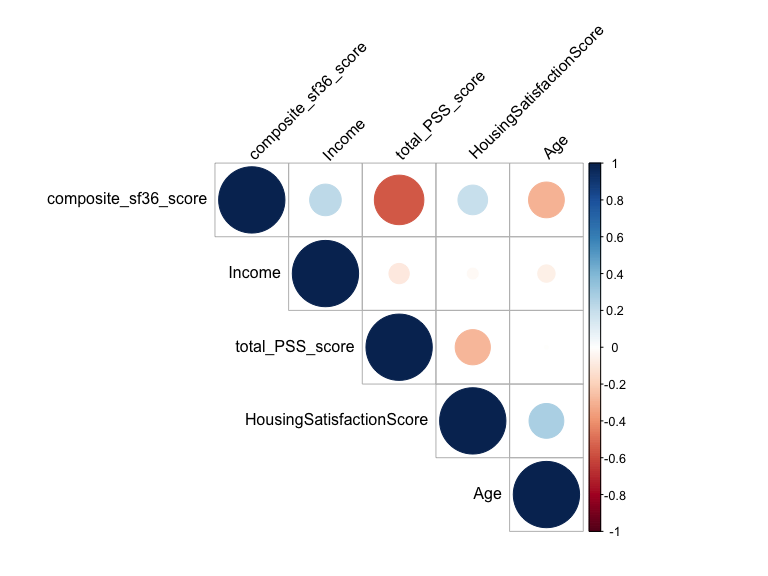
\includegraphics[width=0.9\linewidth]{Data-Cleaning-Coding_files/figure-latex/unnamed-chunk-49-1}


\end{document}
